% Options for packages loaded elsewhere
\PassOptionsToPackage{unicode}{hyperref}
\PassOptionsToPackage{hyphens}{url}
\PassOptionsToPackage{dvipsnames,svgnames*,x11names*}{xcolor}
%
\documentclass[
  a4paper, 12pt]{article}
\usepackage{lmodern}
\usepackage{amssymb,amsmath}
\usepackage{ifxetex,ifluatex}
\ifnum 0\ifxetex 1\fi\ifluatex 1\fi=0 % if pdftex
  \usepackage[T1]{fontenc}
  \usepackage[utf8]{inputenc}
  \usepackage{textcomp} % provide euro and other symbols
\else % if luatex or xetex
  \usepackage{unicode-math}
  \defaultfontfeatures{Scale=MatchLowercase}
  \defaultfontfeatures[\rmfamily]{Ligatures=TeX,Scale=1}
\fi
% Use upquote if available, for straight quotes in verbatim environments
\IfFileExists{upquote.sty}{\usepackage{upquote}}{}
\IfFileExists{microtype.sty}{% use microtype if available
  \usepackage[]{microtype}
  \UseMicrotypeSet[protrusion]{basicmath} % disable protrusion for tt fonts
}{}
\makeatletter
\@ifundefined{KOMAClassName}{% if non-KOMA class
  \IfFileExists{parskip.sty}{%
    \usepackage{parskip}
  }{% else
    \setlength{\parindent}{0pt}
    \setlength{\parskip}{6pt plus 2pt minus 1pt}}
}{% if KOMA class
  \KOMAoptions{parskip=half}}
\makeatother
\usepackage{xcolor}
\IfFileExists{xurl.sty}{\usepackage{xurl}}{} % add URL line breaks if available
\IfFileExists{bookmark.sty}{\usepackage{bookmark}}{\usepackage{hyperref}}
\hypersetup{
  pdftitle={Modelos mistos na Engenharia de Avaliações},
  pdfauthor={Luiz Fernando Palin Droubi; Carlos Augusto Zilli; Norberto Hoccheim},
  colorlinks=true,
  linkcolor=red,
  filecolor=Maroon,
  citecolor=green,
  urlcolor=magenta,
  pdfcreator={LaTeX via pandoc}}
\urlstyle{same} % disable monospaced font for URLs
\usepackage[left=3.5cm,right=2.5cm,top=2.5cm,bottom=2.5cm]{geometry}
\usepackage{longtable,booktabs}
% Correct order of tables after \paragraph or \subparagraph
\usepackage{etoolbox}
\makeatletter
\patchcmd\longtable{\par}{\if@noskipsec\mbox{}\fi\par}{}{}
\makeatother
% Allow footnotes in longtable head/foot
\IfFileExists{footnotehyper.sty}{\usepackage{footnotehyper}}{\usepackage{footnote}}
\makesavenoteenv{longtable}
\usepackage{graphicx,grffile}
\makeatletter
\def\maxwidth{\ifdim\Gin@nat@width>\linewidth\linewidth\else\Gin@nat@width\fi}
\def\maxheight{\ifdim\Gin@nat@height>\textheight\textheight\else\Gin@nat@height\fi}
\makeatother
% Scale images if necessary, so that they will not overflow the page
% margins by default, and it is still possible to overwrite the defaults
% using explicit options in \includegraphics[width, height, ...]{}
\setkeys{Gin}{width=\maxwidth,height=\maxheight,keepaspectratio}
% Set default figure placement to htbp
\makeatletter
\def\fps@figure{htbp}
\makeatother
\setlength{\emergencystretch}{3em} % prevent overfull lines
\providecommand{\tightlist}{%
  \setlength{\itemsep}{0pt}\setlength{\parskip}{0pt}}
\setcounter{secnumdepth}{5}
\usepackage[brazil]{babel}
\usepackage{amsmath}
\usepackage{graphicx}
\usepackage{float}
\usepackage{subfig}
\usepackage{caption}
\usepackage{lastpage}
\usepackage{rotating}
\usepackage{mathrsfs}
\usepackage{bm}
\usepackage{dcolumn}
\setlength{\parindent}{1.25cm} % Default is 15pt.
\usepackage{indentfirst}
% \usepackage{helvet}
% \renewcommand{\familydefault}{\sfdefault}
% \usepackage{newtxtext,newtxmath} % mais nova para Times.
%\usepackage{mathptmx} % para Times New Roman (preferível newtxtext)
% \usepackage{Times} % para Times New Roman (obsoleto)
\usepackage{fontspec} % para Arial e/ou Times (xelatex ou luatex)
\setmainfont{Arial}
\newcommand{\pkg}[1]{{\normalfont\fontseries{b}\selectfont #1}}
\let\proglang=\textsf
\let\code=\texttt
\usepackage{fancyhdr}
% Turn on the style
\pagestyle{fancy}
% Clear the header and footer
\fancyhead{}
\fancyfoot{}
% Set the right side of the footer to be the page number
\fancyfoot[R]{\thepage~/~\pageref{LastPage}}
\usepackage{booktabs}
\usepackage{longtable}
\usepackage{array}
\usepackage{multirow}
\usepackage{wrapfig}
\usepackage{float}
\usepackage{colortbl}
\usepackage{pdflscape}
\usepackage{tabu}
\usepackage{threeparttable}
\usepackage{threeparttablex}
\usepackage[normalem]{ulem}
\usepackage{makecell}
\usepackage{xcolor}

\title{Modelos mistos na Engenharia de Avaliações}
\usepackage{etoolbox}
\makeatletter
\providecommand{\subtitle}[1]{% add subtitle to \maketitle
  \apptocmd{\@title}{\par {\large #1 \par}}{}{}
}
\makeatother
\subtitle{Possibilidades e aplicações}
\author{Luiz Fernando Palin Droubi\footnote{SPU/SC,
  \href{mailto:luiz.droubi@planejamento.gov.br}{\nolinkurl{luiz.droubi@planejamento.gov.br}}} \and Carlos Augusto Zilli\footnote{IFSC,
  \href{mailto:carloszilli@hotmail.com}{\nolinkurl{carloszilli@hotmail.com}}} \and Norberto Hoccheim\footnote{UFSC,
  \href{mailto:hochheim@gmail.com}{\nolinkurl{hochheim@gmail.com}}}}
\date{27/08/2020}

\begin{document}
\maketitle

\hypertarget{introduuxe7uxe3o}{%
\section{Introdução}\label{introduuxe7uxe3o}}

Na Engenharia de Avaliaçãoes, assim como em diversos ramos das ciências
sociais, a abordagem padrão para lidar com a heteregoneidade amostral é
a modelagem com efeitos fixos. Este tipo de abordagem permite a
segregação dos dados da amostra em diferentes agrupamentos, no entanto,
ela não

\hypertarget{revisuxe3o-bibliogruxe1fica}{%
\section{Revisão Bibliográfica}\label{revisuxe3o-bibliogruxe1fica}}

A análise de dados multinível é usualmente feita, nos diversos ramos da
ciência por meio de modelos de efeitos fixos. No entanto, de acordo com
Bell \emph{et al.} (\protect\hyperlink{ref-bell2019}{2019}, p. 1052), os
modelos mistos bem especificados oferecem uma abordagem muito mais
completa destes tipos de dados do que a modelagem por efeitos fixos.

Segundo Bell \emph{et al.} (\protect\hyperlink{ref-bell2019}{2019}, p.
1051), existe uma confusão na literatura a respeito de modelos mistos,
no que tange à aglutinação em uma modelagem de diversos tipos de
efeitos, fixos e aleatórios, sendo que os modelos mistos mais complexos
tem sido chamados, erroneamente, de modelos híbridos.

\hypertarget{modelagem-por-efeitos-fixos}{%
\subsection{Modelagem por efeitos
fixos}\label{modelagem-por-efeitos-fixos}}

A modelagem por efeitos fixos é frequentemente aplicada na Engenharia de
Avaliações, assim como em diversas outras áreas da ciência (BELL et al.,
\protect\hyperlink{ref-bell2019}{2019}, p. 1057), apesar desta
terminologia não ser normalmente empregada. Um modelo de efeitos fixos
nada mais é do que um modelo em que a heterogeneidade da amostra é
``saneada'' através da inclusão de variáveis \emph{dummies}\footnote{Neste
  trabalho as variáveis dicotômicas em grupo serão tratadas simplesmente
  pelo termo em inglês \emph{dummies}.} representando cada agrupamento
de dados. Após a inclusão destas variáveis saneando a amostra, ou seja,
tornando-a homogênea, a estimação é feita pelo métodos dos mínimos
quadrados ordinários.

A modelagem por efeitos fixos pode ser escrita conforme a equação
\ref{eq:fixef}, onde a variância entre os agrupamentos de dados
(variância de nível mais alto) é modelada através de variáveis
\emph{dummies} \(D_j\) (BELL; JONES,
\protect\hyperlink{ref-bell2015}{2015}, p. 138):

\begin{equation} \label{eq:fixef}
y_{ij} = \sum_{j=1}^{j}\beta_{0j}D_j + \beta_1 x_{ij} + \epsilon_{ij}
\end{equation}

No entanto, uma outra maneira mais conveniente - para a comparação que
se pretende de escrever a formulação de efeitos fixos, equivalente à
primeira, pode ser vista na equação \ref{eq:fixef2} (BELL et al.,
\protect\hyperlink{ref-bell2019}{2019}, p. 1058):

\begin{equation} \label{eq:fixef2}
y_{ij} = \beta_1 (x_{ij} - \bar{x}_j) + (\upsilon_i + \epsilon_{ij}) 
\end{equation}

Onde \(\upsilon_i\) é um termo discreto para cada agrupamento de
dados\footnote{O termo \(\upsilon_i\) é o intercepto de cada
  agrupamento, quando se ajusta um modelo sem intercepto.}. Os índices
\(i\) e \(j\) se referem aos dois níveis de análise: \(i\), neste caso,
representa o nível dos indivíduos e \(j\) o nível dos agrupamentos.
\(\epsilon_{ij}\) é um termo de erro aleatório com distribuição
supostamente normal, média zero e desvio-padrão \(\sigma_{\epsilon}^2\).

Na prática, no entanto, a formulação acima raramente é utilizada, pois
perde-se um grau de liberdade na estimação de um intercepto para cada
bairro, quando se pode utilizar um nível de referência e estimar apenas
a diferença entre os níveis de cada agrupamento em relação a este nível
de referência, como ilustrado na equação \ref{eq:fixef3} (BELL et al.,
\protect\hyperlink{ref-bell2019}{2019}, p. 1058).

\begin{equation} \label{eq:fixef3}
(y_{ij} - \bar{y}_i) = \beta_1 (x_{ij} - \bar{x}_j) + (\epsilon_{ij}) 
\end{equation}

\hypertarget{modelagem-por-efeitos-mistos}{%
\subsection{Modelagem por efeitos
mistos}\label{modelagem-por-efeitos-mistos}}

Existem diversas maneiras de utilização da modelagem por efeitos mistos.
Neste trabalho apresenta-se as diversas possibilidades, desde a
abordagem mais simples, que possibilita uma comparação direta com o
modelo de efeitos fixos, muito conhecido na Engenharia de Avaliações,
até a abordagem mais complexa, a formulação REWB

\hypertarget{modelo-de-efeitos-mistos-simples}{%
\subsubsection{Modelo de efeitos mistos
simples}\label{modelo-de-efeitos-mistos-simples}}

A modelagem por efeitos mistos considera, além dos efeitos fixos, um
termo de efeitos aleatórios (BELL et al.,
\protect\hyperlink{ref-bell2019}{2019}, p. 1057). Uma das maneiras de
escrever a formulação de efeitos mistos pode ser vista na equação
\ref{eq:mixef}.

\begin{equation} \label{eq:mixef}
y_{ij} = \beta_0 + \beta_1^{RE} x_{ij} + \beta_2 z_j + (\upsilon_j + \epsilon_{ij}) 
\end{equation}

No caso da equação \ref{eq:mixef}, o termo \(\upsilon_j\) é um termo
estocástico de efeitos aleatórios para os indivíduos, suposto
normalmente distribuído e com média zero, ou seja
\(\upsilon_j \sim N(0, \sigma_{\upsilon}^2)\) (BELL et al.,
\protect\hyperlink{ref-bell2019}{2019}, p. 1055). A variável \(x_{ij}\)
é uma variável de nível 1, variante entre os diferentes agrupamentos e a
variável \(z_j\) é uma variável de nível 2, considerada invariante entre
os agrupamentos. Neste tipo de modelagem estimam-se, além dos
coeficientes das variáveis de nível mais baixo \(\beta_0\) e
\(\beta_1\), o(s) coeficiente(s) da(s) variável(eis) de segundo nível
\(\beta_2\) e os parâmetros \(\sigma_\upsilon^2\) e
\(\sigma_\epsilon^2\), ou seja, as variâncias de primeiro e segundo
nível, respectivamente.

A diferença de nível entre as variáveis pode ser melhor compreendida ao
se dividir a modelagem em dois níveis (alguns autores se referem a este
tipo de modelagem como hierárquica), como pode ser visto nas equações
\ref{eq:micro} e \ref{eq:macro}:

\begin{equation} \label{eq:micro}
y_{ij} = \beta_{0j} + \beta_1^{RE} x_{ij} + \epsilon_{ij} 
\end{equation}

\begin{equation} \label{eq:macro}
\beta_{0j} = \beta_0 + \beta_2 z_{j} + \upsilon_{j} 
\end{equation}

Segundo Bell e Jones (\protect\hyperlink{ref-bell2015}{2015}, pp.
135--136), a equação \ref{eq:micro} é chamada de parte micro, enquanto a
equação \ref{eq:macro} é chamada de parte macro da formulação de efeitos
mistos, que são estimadas em conjunto ao substituir \ref{eq:macro} em
\ref{eq:micro} para se obter o modelo misto da equação \ref{eq:mixef}.

Em suma, para Bell \emph{et al.}
(\protect\hyperlink{ref-bell2019}{2019}, p. 1061), a grande diferença
entre a formulação de efeitos fixos e a formulação de efeitos mistos
está na maneira como as modelagens tratam os agrupamentos de dados, se
de maneira discreta (efeitos fixos) ou de maneira aleatória (efeitos
aleatórios). Enquanto na modelagem de efeitos fixos são adicionadas
variáveis \emph{dummies} discretas para a modelagem dos diferentes
agrupamentos, na modelagem de efeitos aleatórios é considerado que a
diferença entre os dados de diferentes agrupamentos pode ser modelada
por uma variável aleatória normal. Assim, os modelos de efeitos fixos
consomem todos os graus de liberdade do segundo nível hierárquico ,
matando assim a possibilidade de inferências a respeito da variância em
nível mais alto, sendo impossível medir os efeitos de variáveis como
\(z_j\), na equação \ref{eq:mixef} (BELL; JONES,
\protect\hyperlink{ref-bell2015}{2015}, p. 139).

Segundo os autores citados, ainda, esta visão não é unânime: na
econometria, por exemplo, é considerado que a diferença fundamental
entre as modelagens de efeitos fixos e efeitos mistos está de fato na
hipótese considerada pelos modelos mistos de que não há correlação dos
efeitos aleatórios (representados por \(\upsilon_i\)) e os regressores
(\(x_ij\)), o que é permitido na modelagem de efeitos fixos (BELL et
al., \protect\hyperlink{ref-bell2019}{2019}, p. 1060).

Este tipo de modelagem ainda pode ser facilmente estendida para
incorporar outros níveis hierárquicos mais altos, assim como
variabilidade não apenas para os interceptos, mas também para os
coeficientes das variáveis explicativas (BELL et al.,
\protect\hyperlink{ref-bell2019}{2019}, p. 1052).

\hypertarget{formulauxe7uxe3o-de-mundlak}{%
\subsubsection{Formulação de
Mundlak}\label{formulauxe7uxe3o-de-mundlak}}

Uma maneira mais adequada de escrever a formulação de modelos mistos
consiste na separação dos efeitos dentro dos agrupamentos dos efeitos
entre os agrupamentos, o que é conhecido na literatura por formulação
\emph{within-between}. Esta formulação é a mais genérica, capaz de
modelar diversos efeitos e é particularmente interessante na análise de
dados em painéis ou séries temporais, e será apresentada no próximo
item. No caso de dados em seção transversal, no entanto, esta formulação
pode ser ligeiramente modificada como mostrado na equação
\ref{eq:mundlak}, o que é conhecido na literatura como formulação de
Mundlak (BELL et al., \protect\hyperlink{ref-bell2019}{2019}, p. 1055):

\begin{equation} \label{eq:mundlak}
y_{ij} = \beta_0 + \beta_{1W} x_{ij} + \beta_{2C}\bar{x}_i+ \beta_3 z_i + (\upsilon_i + \epsilon_{ij}) 
\end{equation}

Segundo BELL et al. (\protect\hyperlink{ref-bell2019}{2019}, p. 1055),
na formulação de Mundlak o efeito contextual, representado na equação
\ref{eq:mundlak} pelo termo \(\beta_{2C}\), é de interesse. O que este
termo modela é como uma mudança de contexto (no caso da Engenharia de
Avaliações, uma mudança de bairros, por exemplo), afeta o valor de um
indivíduo (neste caso, imóveis).

Na prática, segundo BELL et al. (\protect\hyperlink{ref-bell2019}{2019},
p. 1057), os modelos de Mundlak e os modelos de efeitos fixos estimarão
exatamente os mesmos valores para os coeficientes de efeitos dentro dos
agrupamentos (\emph{within effects}), representado na formulação acima
pelo termo \(\beta_{1W}\).

\hypertarget{formulauxe7uxe3o-within-between}{%
\subsubsection{Formulação
Within-Between}\label{formulauxe7uxe3o-within-between}}

A formulação \emph{within-between} (REWB) é a mais genérica, normalmente
utilizada para o ajuste de modelos com dados em painéis, onde os
indivíduos (\(i\)) são medidos em múltiplas ocasiões (\(t\)). Esta
formulação é capaz de distinguir entre os efeitos dentro (\emph{within
effects}) e entre (\emph{between effects}) cada agrupamento.

Na equação \ref{eq:rewb} (BELL et al.,
\protect\hyperlink{ref-bell2019}{2019}, p. 1055) então, os dados estão
agrupados em painéis, não em unidades geográficas, como na formulação de
Mundlak apresentada no item anterior.

\begin{equation} \label{eq:rewb}
y_{it} = \beta_0 + \beta_{1W} (x_{it} - \bar{x}_i) + \beta_{2B}\bar{x}_i+ \beta_3 z_i + (\upsilon_i + \epsilon_{it}) 
\end{equation}

Onde \(\beta_{1W}\) representa o efeito médio entre os indivíduos dentro
(\emph{within}) dos agrupamentos e \(\beta_{2B}\) representa o efeito
entre (\emph{between}) os agrupamentos. No caso de dados em paínéis,
\(\beta_{1W}\) representa o efeito num período e \(\beta_{2B}\)
representa o efeito entre os períodos para a variável não-estacionária
\(x_{it}\).

É possível ainda a construção de um modelo ainda mais genérico que
permite não apenas a modelagem de interceptos aleatórios mas também a
modelagem de coeficientes aleatórios, como descrito na equação
\ref{eq:rewb2}:

\begin{equation} \label{eq:rewb2}
y_{it} = \mu + \beta_{1W} (x_{it} - \bar{x}_i) + \beta_{2B}\bar{x}_i+ 
\beta_3 z_i + \upsilon_{i0} + \upsilon_{i1} (x_{it} - \bar{x}_i) + \epsilon_{it0} 
\end{equation}

Onde o termo \(\upsilon_{i0}\) está relacionado à aleatoriedade do
intercepto e o termo \(\upsilon_{i1}\) está relacionado à aleatoriedade
do coeficiente da variável \(x\).

\hypertarget{considerauxe7uxf5es-sobre-a-pertinuxeancia-de-utilizauxe7uxe3o-de-cada-modelagem}{%
\subsection{Considerações sobre a pertinência de utilização de cada
modelagem}\label{considerauxe7uxf5es-sobre-a-pertinuxeancia-de-utilizauxe7uxe3o-de-cada-modelagem}}

Segundo BELL; JONES (\protect\hyperlink{ref-bell2015}{2015}, p. 143), um
modelo de efeitos fixos pode ser visto como uma forma de modelo de
efeitos mistos onde a variância nos níveis mais altos é restringida, de
maneira que para BELL; JONES (\protect\hyperlink{ref-bell2015}{2015}) os
modelos de efeitos mistos são muito mais interessantes do que os modelos
de efeitos fixos, já que além de propiciarem todas as informações que os
modelos de efeitos fixos propriciam, eles ainda tem possibilidade de ir
além e fornecer outras informações que os modelos de efeitos fixos não
fornecem, como a separação dos efeitos de uma variável entre (efeito
\emph{between}) os agrupamentos e dentro (efeito \emph{within}) dos
agrupramentos. Para BELL et al. (\protect\hyperlink{ref-bell2019}{2019},
p. 1060), para o efeito dentro dos agrupamentos (\emph{within effect}),
os resultados estimados pela formulação REWB ou pela formulação de
Mundlak serão rigorosamente os mesmos obtidos pelo modelo de efeitos
fixos. No entanto, enquanto os modelos de REWB e de Munlak fornecem
informações a respeitos dos efeitos entre os agrupamentos (\emph{between
effects}), os modelos de efeitos fixos não são capazes de fornecer
qualquer informação a este respeito.

Deve ser observado que a hipótese de modelar os diversos agrupamentos
como uma variável aleatória é razoável apenas quando o número de
agrupamentos for grande o suficiente. Para poucos agrupamentos, a
modelagem por efeitos fixos ainda parece ser mais adequada (ver BELL et
al., \protect\hyperlink{ref-bell2019}{2019}, p. 1071).

Também deve ser observado que a utilização da formulação simples para
modelos mistos, como a da equação \ref{eq:mixef}, como muitas vezes se
encontra na prática (ver CICHULSKA; CELLMER,
\protect\hyperlink{ref-polonia}{2018}), não é tão interessante como a
aplicação das modelagens REWB e de Mundlak. No entanto, a aplicação da
formulação REWB e de Mundlak só faz sentido se houver efetivamente uma
diferença entre os efeitos dentro e entre os agrupamentos. Caso
\(\beta_{1W} = \beta_{2B}\) (REWB) ou \(\beta_{2C} = 0\) (Mundlak), não
faz sentido utilizar estas formulações e a formulação simples de efeitos
mistos (equação \ref{eq:mixef}) deve ser a adotada (BELL et al.,
\protect\hyperlink{ref-bell2019}{2019}, p. 1058).

\hypertarget{considerauxe7uxf5es-a-respeito-da-estimauxe7uxe3o-em-modelos-mistos}{%
\subsection{Considerações a respeito da estimação em modelos
mistos}\label{considerauxe7uxf5es-a-respeito-da-estimauxe7uxe3o-em-modelos-mistos}}

Segundo CLARK (\protect\hyperlink{ref-clark2019shrinkage}{2019}), a
estimação em modelos mistos é feita à partir do encolhimento.

\hypertarget{estudo-de-caso}{%
\section{Estudo de Caso}\label{estudo-de-caso}}

Para o estudo de caso foi utilizada a implementação do pacote \pkg{lme4}
(BATES et al., \protect\hyperlink{ref-Bates}{2015}) no \proglang{R},
versão 4.0.2 (R CORE TEAM, \protect\hyperlink{ref-R}{2020}).

\hypertarget{criauxe7uxe3o-de-dados-via-simulauxe7uxe3o}{%
\subsection{Criação de dados via
simulação}\label{criauxe7uxe3o-de-dados-via-simulauxe7uxe3o}}

Foram criados 550 dados de lotes, divididos igualmente em 11 bairros, a
partir de simulação com o auxílio do software \textbf{R}.

Os dados foram criados conforme parâmetros da tabela 1:

\begin{longtable}[]{@{}lrcrc@{}}
\toprule
\begin{minipage}[b]{0.18\columnwidth}\raggedright
Variável\strut
\end{minipage} & \begin{minipage}[b]{0.12\columnwidth}\raggedleft
Tipo\strut
\end{minipage} & \begin{minipage}[b]{0.11\columnwidth}\centering
Distribuição\strut
\end{minipage} & \begin{minipage}[b]{0.25\columnwidth}\raggedleft
Parâmetros\strut
\end{minipage} & \begin{minipage}[b]{0.21\columnwidth}\centering
Obs\strut
\end{minipage}\tabularnewline
\midrule
\endhead
\begin{minipage}[t]{0.18\columnwidth}\raggedright
Área (\(A\))\strut
\end{minipage} & \begin{minipage}[t]{0.12\columnwidth}\raggedleft
Quantitativa\strut
\end{minipage} & \begin{minipage}[t]{0.11\columnwidth}\centering
Normal\strut
\end{minipage} & \begin{minipage}[t]{0.25\columnwidth}\raggedleft
\(\mu = 400, \sigma = 50\)\strut
\end{minipage} & \begin{minipage}[t]{0.21\columnwidth}\centering
-\strut
\end{minipage}\tabularnewline
\begin{minipage}[t]{0.18\columnwidth}\raggedright
Bairro\strut
\end{minipage} & \begin{minipage}[t]{0.12\columnwidth}\raggedleft
Qualitativa\strut
\end{minipage} & \begin{minipage}[t]{0.11\columnwidth}\centering
-\strut
\end{minipage} & \begin{minipage}[t]{0.25\columnwidth}\raggedleft
A a K\strut
\end{minipage} & \begin{minipage}[t]{0.21\columnwidth}\centering
-\strut
\end{minipage}\tabularnewline
\begin{minipage}[t]{0.18\columnwidth}\raggedright
Áreas Verdes (\(A_V\))\strut
\end{minipage} & \begin{minipage}[t]{0.12\columnwidth}\raggedleft
Quantitativa\strut
\end{minipage} & \begin{minipage}[t]{0.11\columnwidth}\centering
Uniforme\strut
\end{minipage} & \begin{minipage}[t]{0.25\columnwidth}\raggedleft
\(\mu = 0,2 \quad a \quad 0,70\)\strut
\end{minipage} & \begin{minipage}[t]{0.21\columnwidth}\centering
Um valor para cada bairro\strut
\end{minipage}\tabularnewline
\begin{minipage}[t]{0.18\columnwidth}\raggedright
\(\beta_{0}\)\strut
\end{minipage} & \begin{minipage}[t]{0.12\columnwidth}\raggedleft
Coeficiente\strut
\end{minipage} & \begin{minipage}[t]{0.11\columnwidth}\centering
Discreta\strut
\end{minipage} & \begin{minipage}[t]{0.25\columnwidth}\raggedleft
2000\strut
\end{minipage} & \begin{minipage}[t]{0.21\columnwidth}\centering
-\strut
\end{minipage}\tabularnewline
\begin{minipage}[t]{0.18\columnwidth}\raggedright
\(\upsilon\)\strut
\end{minipage} & \begin{minipage}[t]{0.12\columnwidth}\raggedleft
Termo de erro\strut
\end{minipage} & \begin{minipage}[t]{0.11\columnwidth}\centering
Normal\strut
\end{minipage} & \begin{minipage}[t]{0.25\columnwidth}\raggedleft
\(\mu = 0, \sigma = 50\)\strut
\end{minipage} & \begin{minipage}[t]{0.21\columnwidth}\centering
-\strut
\end{minipage}\tabularnewline
\begin{minipage}[t]{0.18\columnwidth}\raggedright
\(\beta_{0j}\)\strut
\end{minipage} & \begin{minipage}[t]{0.12\columnwidth}\raggedleft
Coeficiente\strut
\end{minipage} & \begin{minipage}[t]{0.11\columnwidth}\centering
Não definida\strut
\end{minipage} & \begin{minipage}[t]{0.25\columnwidth}\raggedleft
\(\beta_0 + 3000A_V + \upsilon\)\strut
\end{minipage} & \begin{minipage}[t]{0.21\columnwidth}\centering
-\strut
\end{minipage}\tabularnewline
\begin{minipage}[t]{0.18\columnwidth}\raggedright
\(\epsilon\)\strut
\end{minipage} & \begin{minipage}[t]{0.12\columnwidth}\raggedleft
Termo de erro\strut
\end{minipage} & \begin{minipage}[t]{0.11\columnwidth}\centering
Normal\strut
\end{minipage} & \begin{minipage}[t]{0.25\columnwidth}\raggedleft
\(\mu = 0, \sigma = 100\)\strut
\end{minipage} & \begin{minipage}[t]{0.21\columnwidth}\centering
-\strut
\end{minipage}\tabularnewline
\begin{minipage}[t]{0.18\columnwidth}\raggedright
Valor Unitário (\(VU\))\strut
\end{minipage} & \begin{minipage}[t]{0.12\columnwidth}\raggedleft
Quantitativa\strut
\end{minipage} & \begin{minipage}[t]{0.11\columnwidth}\centering
Não definida\strut
\end{minipage} & \begin{minipage}[t]{0.25\columnwidth}\raggedleft
\(\beta_{0j} - 3,0 A + \epsilon\)\strut
\end{minipage} & \begin{minipage}[t]{0.21\columnwidth}\centering
-\strut
\end{minipage}\tabularnewline
\bottomrule
\end{longtable}

\hypertarget{anuxe1lise-exploratuxf3ria-dos-dados}{%
\subsection{Análise exploratória dos
dados}\label{anuxe1lise-exploratuxf3ria-dos-dados}}

Na figura \ref{fig:exploratoria} é possível ver os principais gráficos
dos dados gerados.

\begin{figure}[H]

{\centering 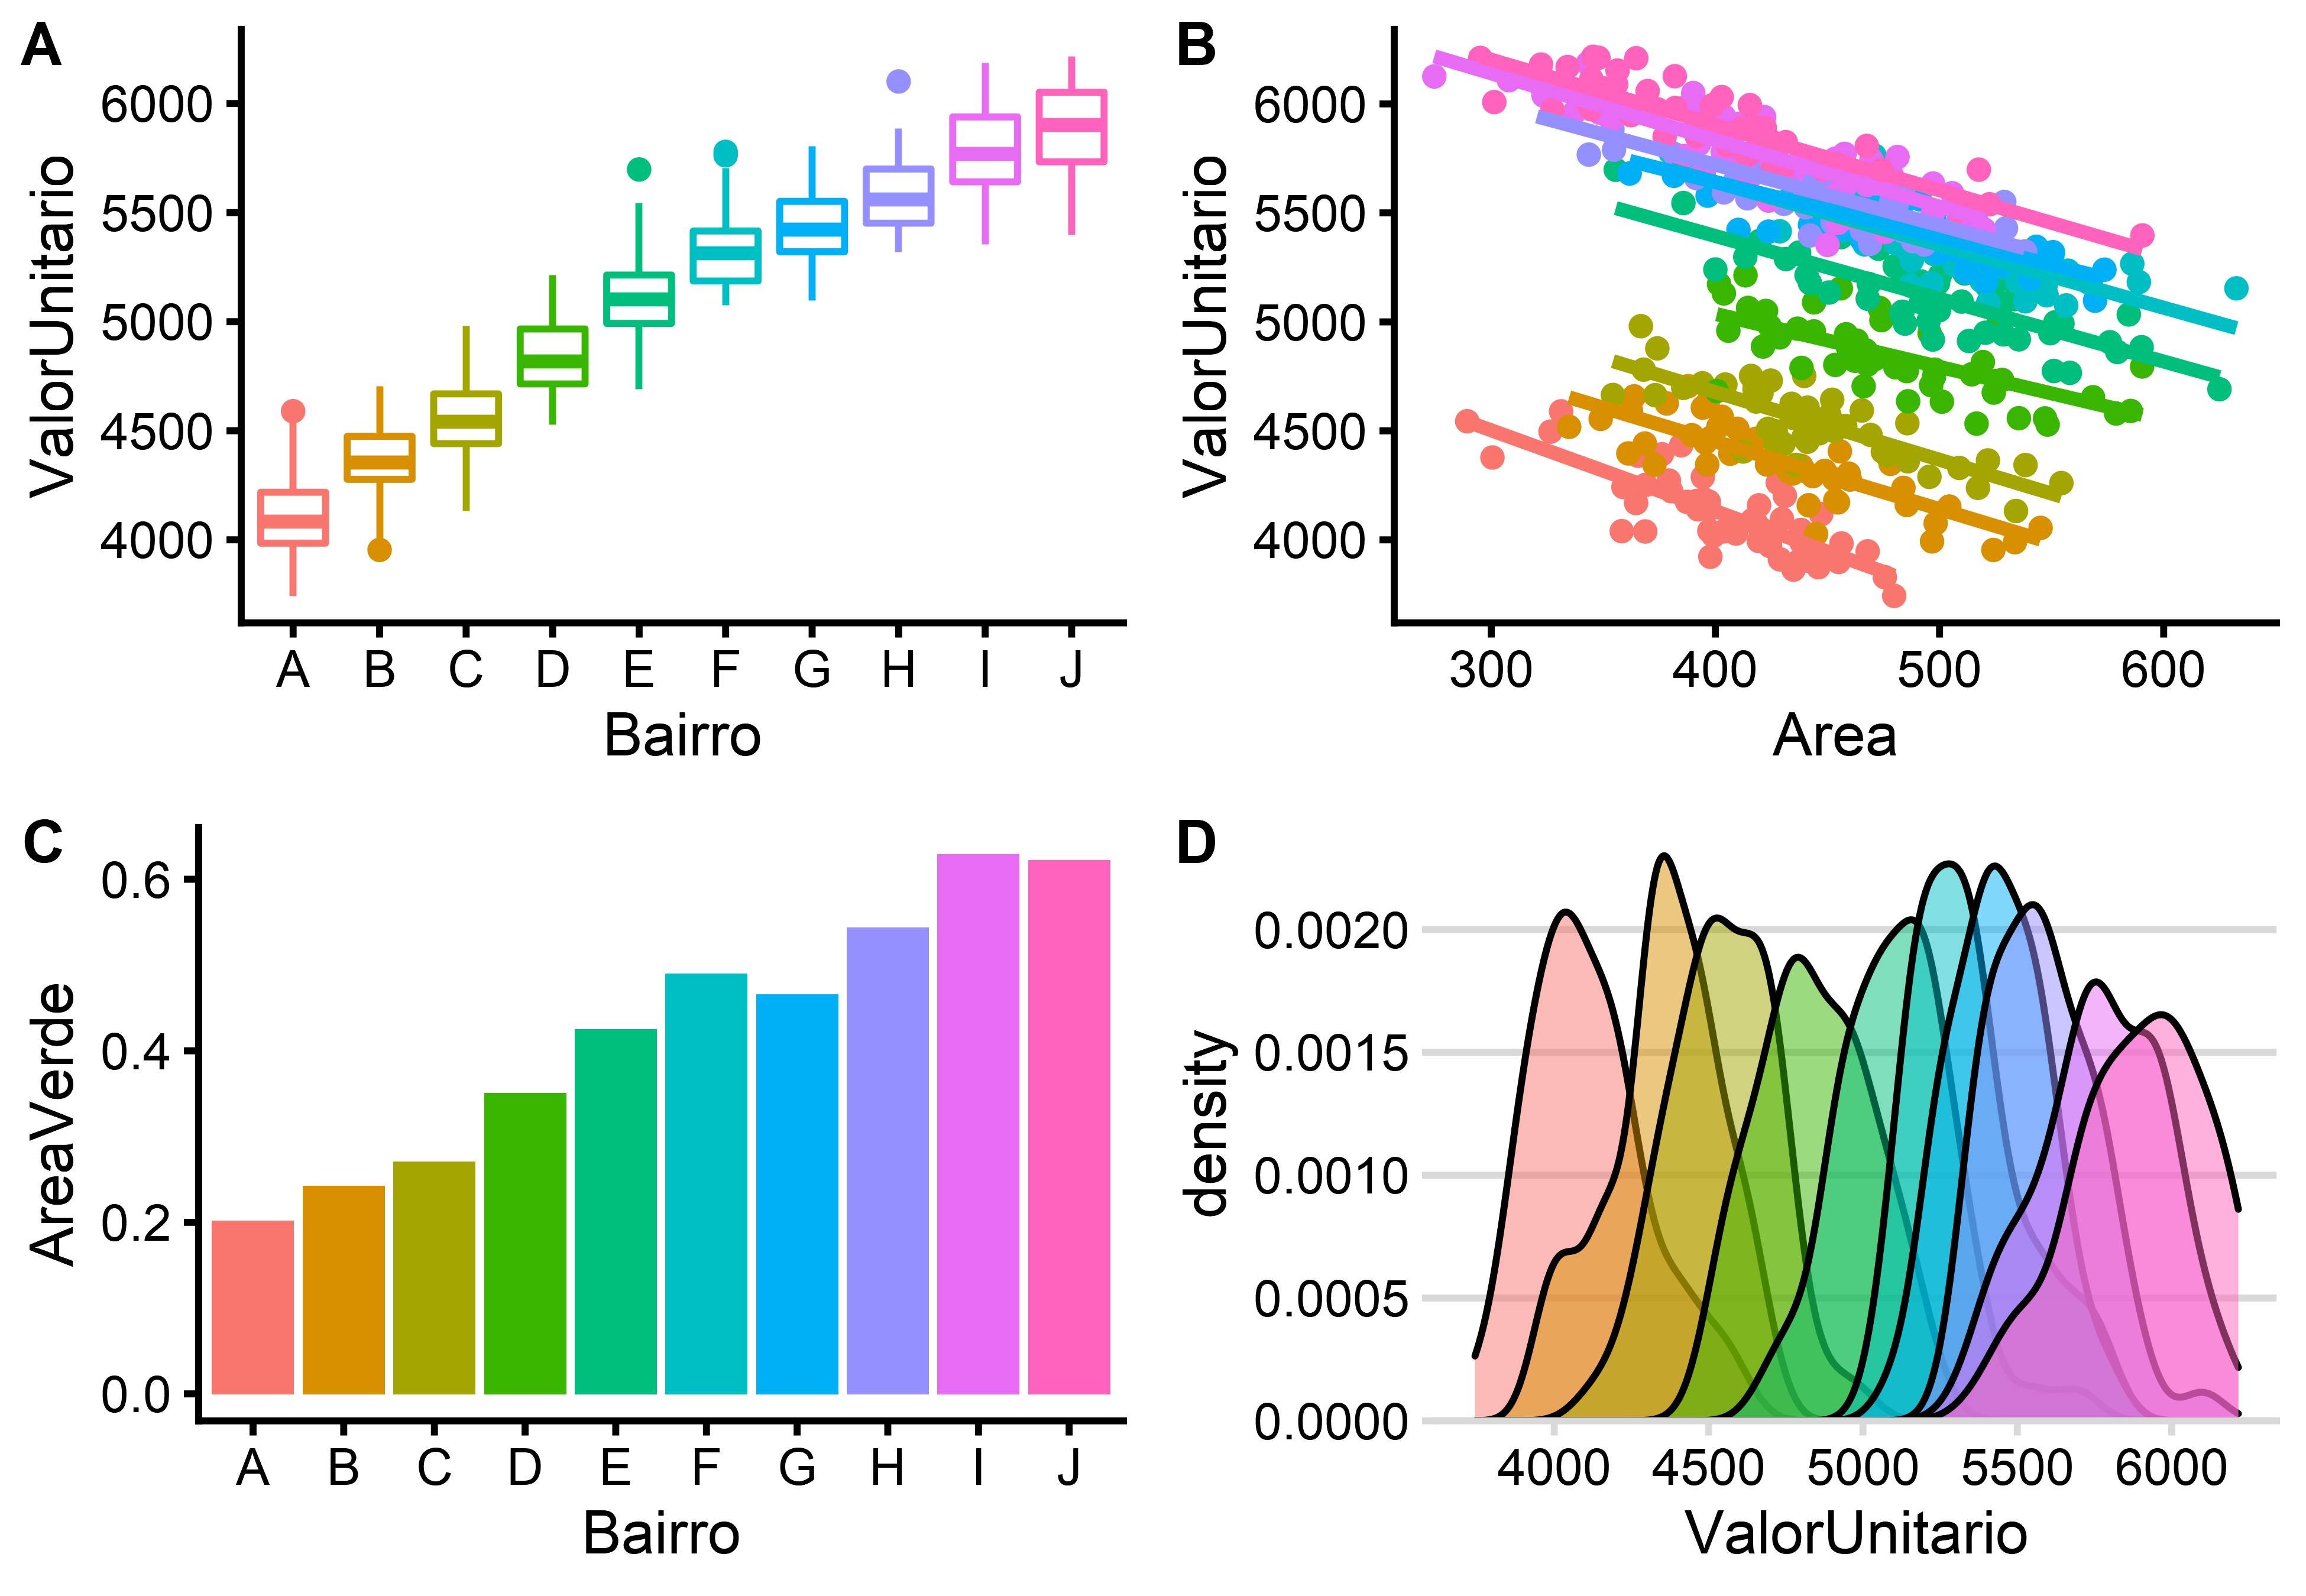
\includegraphics[width=1\linewidth]{images/exploratoria-1} 

}

\caption{Análise exploratória dos dados.}\label{fig:exploratoria}
\end{figure}

\hypertarget{ajuste-de-modelos}{%
\subsection{Ajuste de modelos}\label{ajuste-de-modelos}}

Com os dados gerados foram ajustados um modelo de efeitos fixos e três
modelos mistos: um modelo misto simples, que praticamente equivale ao
modelo de efeitos fixos, um modelo misto com a adição de uma variável de
segundo nível e um modelo misto utilizando-se a formulação de Mundlak.

Para o ajuste do modelo de efeitos fixos foram utilizados todos os dados
gerados, pois não há como prever valores para bairros não contemplados
na amostra em um modelo deste tipo.

\hypertarget{modelo-de-efeitos-fixos}{%
\subsubsection{Modelo de efeitos fixos}\label{modelo-de-efeitos-fixos}}

Com os dados gerados, foi elaborado um modelo de efeitos fixos sem
intercepto, apenas para que fique claro o valor do intercepto aleatório
de cada bairro. Para dar interpretação a estes interceptos aleatórios, a
variável \(Area\) foi centralizada em relação à área de um lote-padrão,
considerado de 400 \(m^2\).\footnote{A centralização de variáveis aqui
  presente não pretende nenhuma separação entre efeitos \emph{within} e
  \emph{between}, mas apenas possibilitar uma interpretação para os
  valores do coeficientes dos interceptos para cada bairro. Ver DROUBI
  et al. (\protect\hyperlink{ref-droubi2019}{2019}) para mais detalhes
  sobre este tipo de centralização.} O modelo é descrito pela equação
\ref{eq:fixefEC}:

\begin{equation} \label{eq:fixefEC}
ValorUnitario = \beta_1 (Area - 400) + \beta_{2i}Bairro_i + \epsilon
\end{equation}

onde \(\beta_{2i}\) são os coeficientes das variáveis dicotômicas em
grupo (\(Bairro_i\)).

\hypertarget{modelos-mistos}{%
\subsubsection{Modelos mistos}\label{modelos-mistos}}

Para o ajuste dos modelos mistos foram removidos os 50 dados relativos
ao bairro H, que foram reservados para serem utilizados posteriormente
para validação dos modelos, mostrando como a previsão de valores em
modelos de efeitos mistos pode ser feita para agrupamentos não
contemplados na amostra.

\hypertarget{modelo-misto-simples}{%
\paragraph{Modelo misto simples}\label{modelo-misto-simples}}

Foi elaborado um modelo misto simples, sem separação de efeitos entre e
dentro dos agrupamentos, de acordo com a equação \ref{eq:simples}:

\begin{equation} \label{eq:simples}
ValorUnitario = \beta_0 + \beta_1 (Area - 400) + \upsilon_i + \epsilon
\end{equation}

Onde \(\upsilon_i\) é uma variável aleatória que foi utilizada para
modelar os diferentes bairros.

\hypertarget{modelo-misto-com-variuxe1veis-de-segundo-nuxedvel}{%
\paragraph{Modelo misto com variáveis de segundo
nível}\label{modelo-misto-com-variuxe1veis-de-segundo-nuxedvel}}

Foi elaborado um modelo misto simples, porém com a presença de variáveis
de segundo nível hierárquico, como demonstrado na equação
\ref{eq:2ndlevel}

\begin{equation} \label{eq:2ndlevel}
ValorUnitario = \beta_0 + \beta_1 (Area - 400) + \beta_2 A_V+ \upsilon_i + \epsilon
\end{equation}

Onde \(A_V\) é uma variável de nível 2 que representa a porcentagem de
áreas verdes em cada bairro, em relação à área total.

\hypertarget{modelo-misto-com-formulauxe7uxe3o-de-mundlak}{%
\paragraph{Modelo misto com formulação de
Mundlak}\label{modelo-misto-com-formulauxe7uxe3o-de-mundlak}}

Finalmente, foi ajusta um modelo com a formulação de Mundlak. Este
modelo foi elaborado de acordo com a formulação exibida na equação
\ref{eq:ECMundlak}:

\begin{equation} \label{eq:ECMundlak}
ValorUnitario = \beta_0 + \beta_1 Area + \beta_{1C} \overline{Area}_i + \beta_2 A_V+ \upsilon_i + \epsilon
\end{equation}

\hypertarget{resultados}{%
\subsection{Resultados}\label{resultados}}

A tabela \ref{tab:fits} mostra as estatísticas básicas dos diversos
modelos mistos (colunas (2), (3) e (4)) comparados aos modelo de efeitos
fixos (coluna (1)).

\begin{table}[H] \centering 
  \caption{Comparacão dos modelos de  efeitos fixos e efeitos mistos.} 
  \label{tab:fits} 
\scriptsize 
\begin{tabular}{@{\extracolsep{5pt}}lcccc} 
\\[-1.8ex]\hline 
\hline \\[-1.8ex] 
 & \multicolumn{4}{c}{\textit{Dependent variable:}} \\ 
\cline{2-5} 
\\[-1.8ex] & \multicolumn{4}{c}{ValorUnitario} \\ 
\\[-1.8ex] & \textit{OLS} & \multicolumn{3}{c}{\textit{linear}} \\ 
 & \textit{} & \multicolumn{3}{c}{\textit{mixed-effects}} \\ 
\\[-1.8ex] & (1) & (2) & (3) & (4)\\ 
\hline \\[-1.8ex] 
 Intercepto &  & 2.116,84 (155,18)$^{***}$ & 788,85 (18,13)$^{***}$ & 1.858,21 (597,46)$^{***}$ \\ 
  (Area - 400) & $-$2,99 (0,09)$^{***}$ & $-$3,00 (0,10)$^{***}$ & $-$3,00 (0,10)$^{***}$ &  \\ 
  Bairro A & 1.379,72 (15,41)$^{***}$ &  &  &  \\ 
  Bairro B & 1.530,98 (15,41)$^{***}$ &  &  &  \\ 
  Bairro C & 1.696,18 (15,42)$^{***}$ &  &  &  \\ 
  Bairro D & 1.891,57 (15,41)$^{***}$ &  &  &  \\ 
  Bairro E & 1.982,52 (15,40)$^{***}$ &  &  &  \\ 
  Bairro F & 2.133,79 (15,41)$^{***}$ &  &  &  \\ 
  Bairro G & 2.313,13 (15,41)$^{***}$ &  &  &  \\ 
  Bairro H & 2.457,33 (15,40)$^{***}$ &  &  &  \\ 
  Bairro I & 2.597,51 (15,41)$^{***}$ &  &  &  \\ 
  Bairro J & 2.741,39 (15,40)$^{***}$ &  &  &  \\ 
  Bairro K & 2.901,56 (15,40)$^{***}$ &  &  &  \\ 
  Area &  &  &  & $-$3,00 (0,10)$^{***}$ \\ 
  Area (between) &  &  &  & 0,32 (1,48) \\ 
  Area Livre &  &  & 3.018,16 (38,65)$^{***}$ & 3.021,14 (43,42)$^{***}$ \\ 
 \hline \\[-1.8ex] 
Observations & 550 & 500 & 500 & 500 \\ 
Log Likelihood &  & $-$3.094,33 & $-$3.055,32 & $-$3.054,02 \\ 
Akaike Inf. Crit. & 6.734,21 & 6.196,66 & 6.120,65 & 6.120,04 \\ 
Bayesian Inf. Crit. & 6.790,23 & 6.213,51 & 6.141,72 & 6.145,33 \\ 
\hline 
\hline \\[-1.8ex] 
\textit{Note:}  & \multicolumn{4}{r}{$^{*}$p$<$0,3; $^{**}$p$<$0,2; $^{***}$p$<$0,1} \\ 
\end{tabular} 
\end{table}

Deve-se notar, primeiramente, que os valores estimados pelo modelo de
efeitos fixos para os interceptos de cada bairro (coluna 1 da tabela
\ref{tab:fits}) são praticamente os mesmos valores obtidos pela
estimação do modelo misto simples, descritos na tabela
\ref{tab:somaitcpt}, onde os valores de referência para cada bairro
foram obtidos através da soma do intercepto global do modelo misto
simples com os interceptos aleatórios do modelo misto simples, que podem
ser visualizados na Figura \ref{fig:dotplot}.

Como se pode notar na Figura \ref{fig:dotplot}, os valores dos
interceptos aleatórios para cada bairro giram em torno de zero, o seu
valor médio. Como o Bairro H (com \(A_L = 0,55\)) foi omitido no ajusto
do modelo, não há valores estimados para os efeitos aleatórios para este
bairro.

\begin{figure}[H]

{\centering 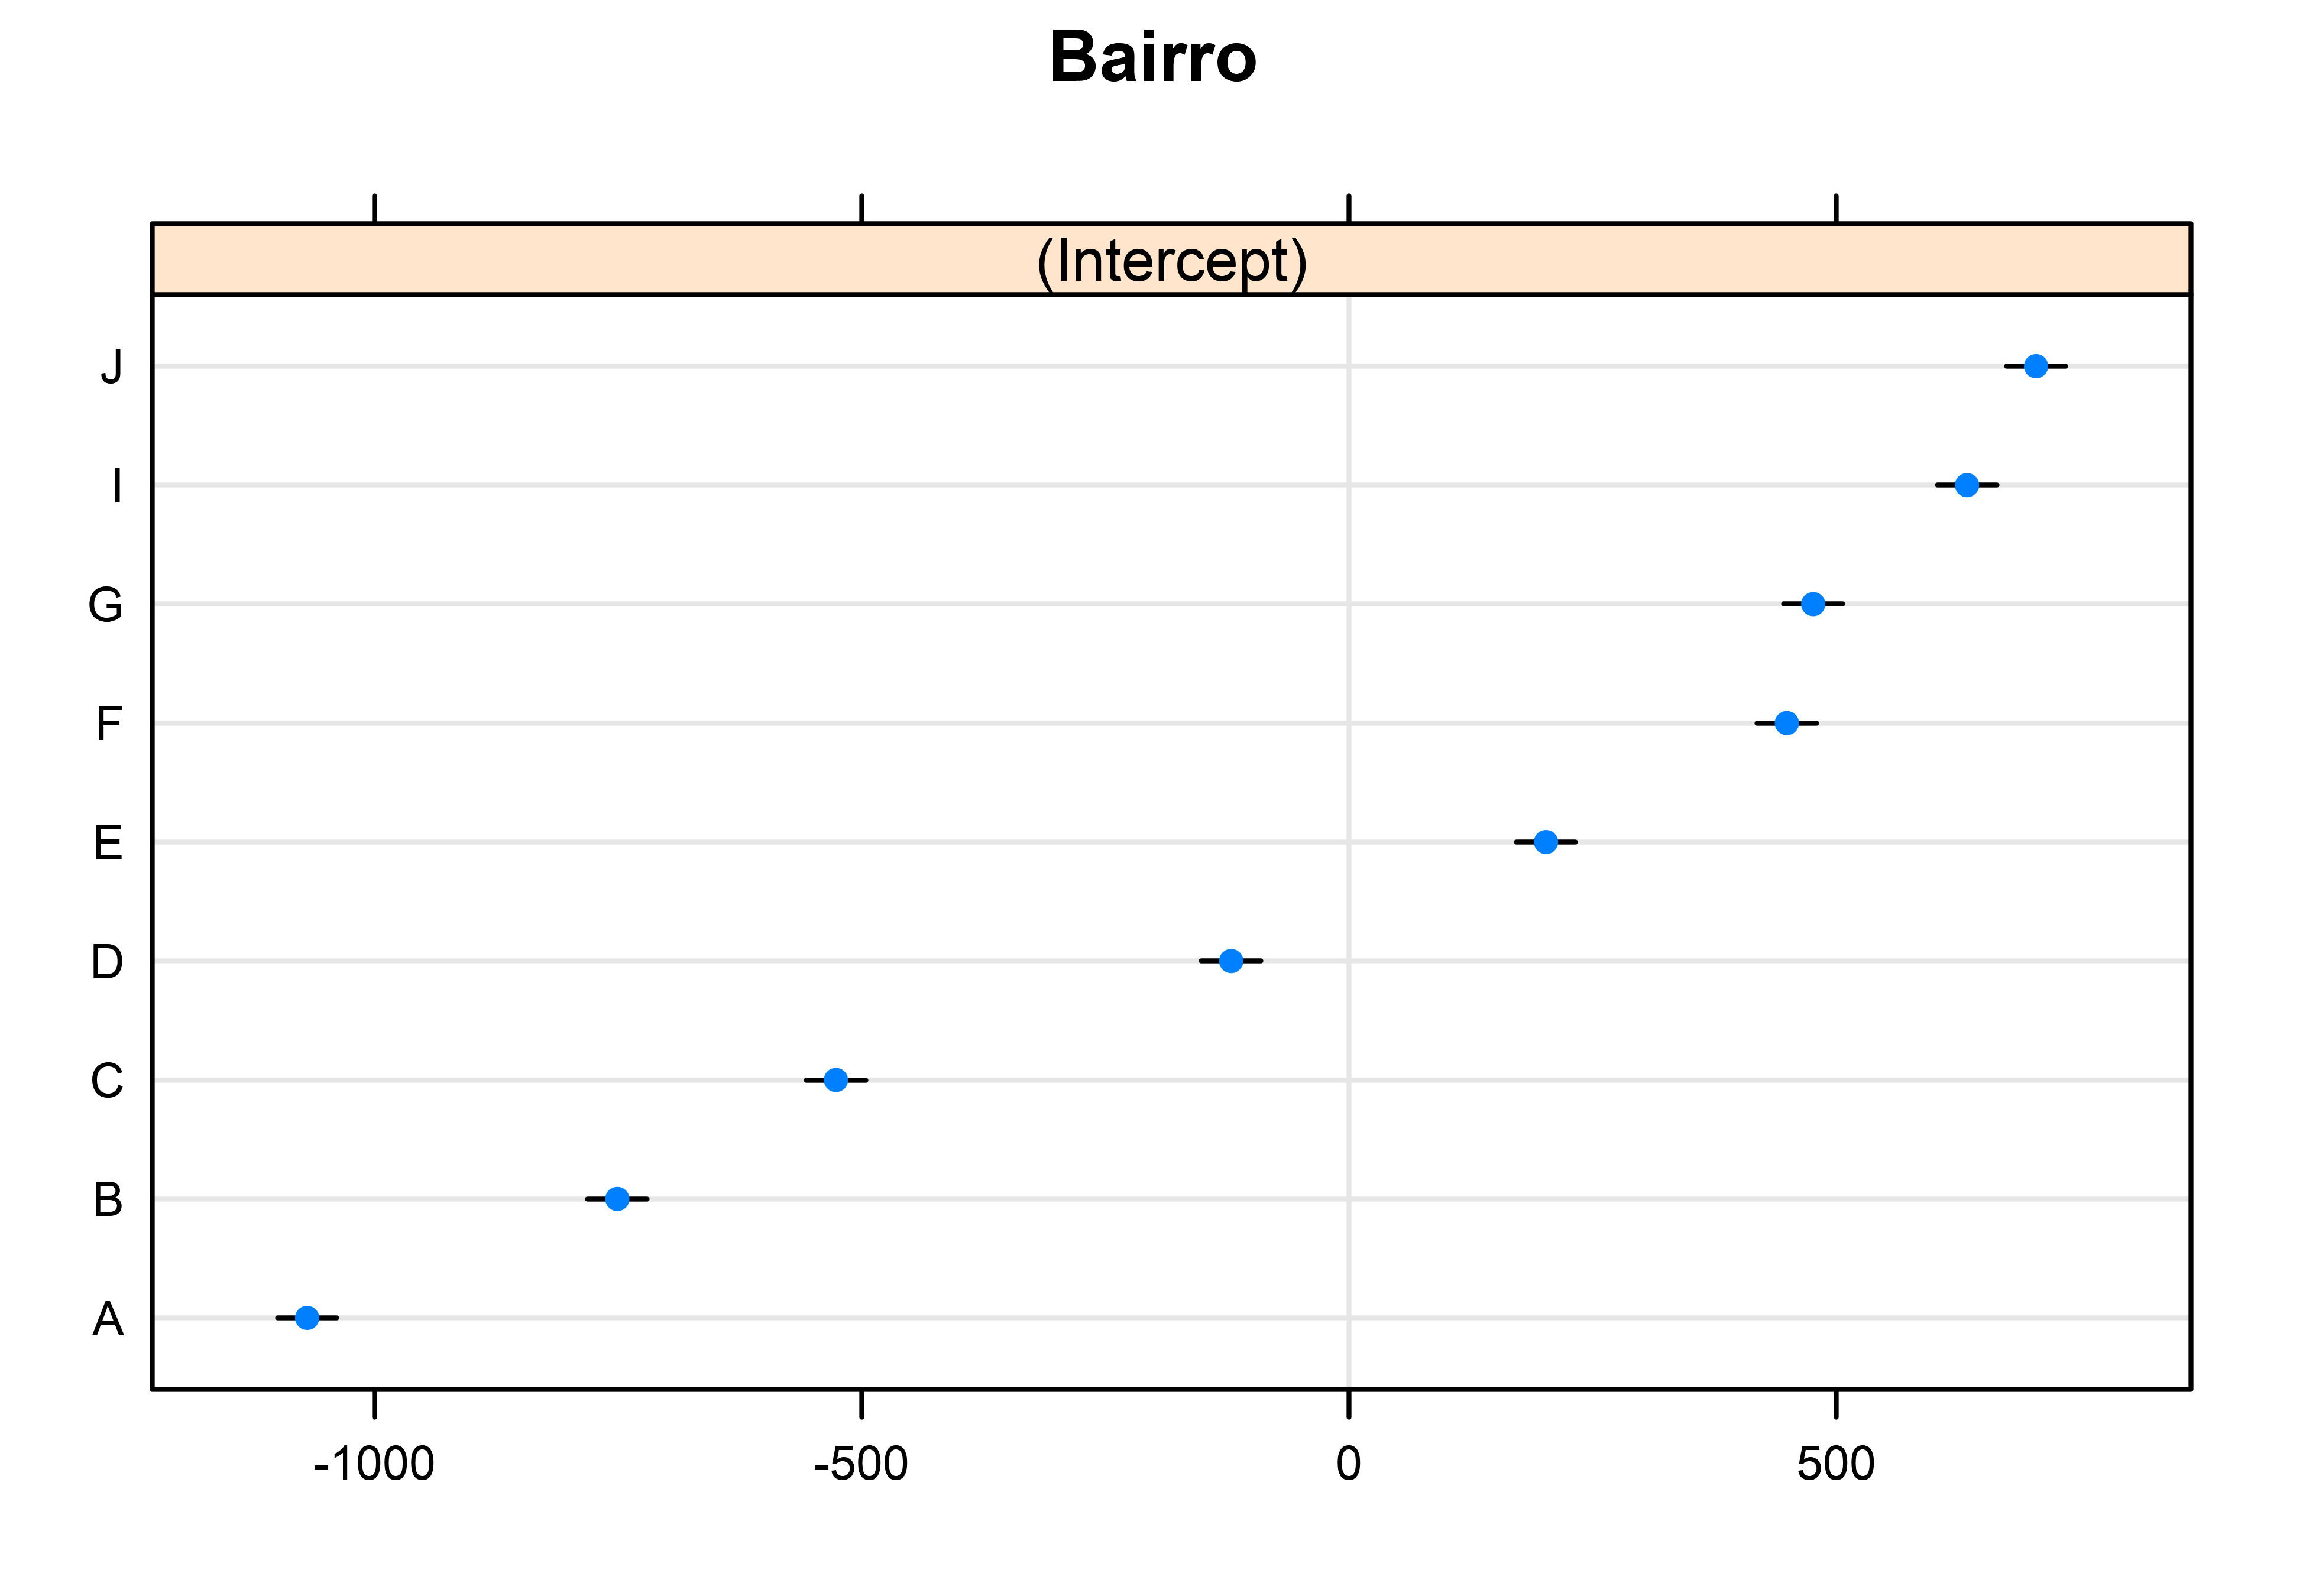
\includegraphics[width=0.7\linewidth]{images/dotplot-1} 

}

\caption{Efeitos aleatórios do modelo.}\label{fig:dotplot}
\end{figure}

\begin{table}[H]

\caption{\label{tab:somaitcpt}Valores dos interceptos para cada bairro.}
\centering
\fontsize{10}{12}\selectfont
\begin{tabular}[t]{rrrrrrrrrr}
\toprule
A & B & C & D & E & F & G & I & J & K\\
\midrule
\rowcolor{gray!6}  -736,4 & -585,2 & -420,3 & -225 & -134,2 & 17 & 196,1 & 480,2 & 623,9 & 783,9\\
\bottomrule
\end{tabular}
\end{table}

A ínica informação a mais que se pode extrair do modelo de efeitos
mistos é a componente de variância devido à localidade, separada da
variância ao nível dos imóveis, o que pode ser visto na tabela
\ref{tab:variancias}.

\begin{table}[H]

\caption{\label{tab:variancias}Efeitos randômicos do modelo misto.}
\centering
\begin{tabular}[t]{lrr}
\toprule
grp & vcov & sdcor\\
\midrule
\rowcolor{gray!6}  Bairro & 240.555,13 & 490,46\\
Residual & 12.105,17 & 110,02\\
\bottomrule
\end{tabular}
\end{table}

Pode-se notar que a variância devido à localidade é relevante para o
modelo, haja vista que a variância devido à localidade é maior do que a
variância devido às características dos imóveis.

Nos modelos onde houve a inclusão da variável Área Livre (\(A_L\)), seu
coeficiente foi bem estimado: o valor da influência das áreas verdes,
simulado como aumento R\$ 30,00/m2 a cada ponto percentual a mais de
áreas verdes no bairro do imóvel, foi precisamente estimado.

Para o modelo de Mundlak, a estimação do coeficiente contextual
(\(\beta_{1C}\)) foi insignificante. Isto era esperado, dado que a
variável Área foi simulada da mesma maneira para todos os bairros. Em
outras palavras, a simulação foi feita como se os imóveis em todos os
bairros tivessem a mesma distribuição (normal) com mesma média e
desvio-padrão. Isto dificilmente ocorrerá na prática da elaboração de
PVG's. Aqui pptou-se, porém, por apresentar desta maneira para se
facilitar a compreensão dos modelos.

Deve-se notar a flexibilidade deste tipo de formulação: quando não
existe na realidade o efeito esperado pela formulação, o coeficiente
resultará insignificante. Diz-se em estatística que o modelo degenera,
ou seja, o modelo com a formulação de Mundlak se degenera para uma
formulação mais simples. Basta remover este termo da modelagem para
obter-se o modelo mais correto para o caso. Portanto, na prática,
deve-se partir da formulação mais complexa, no caso a de Mundlak, e
observar se os resultados obtidos são significantes. Caso positivo,
mantem-se o modelo. Caso contrário, descarta-se o termo insignificante.

Essa mesma degeneração ocorre com os modelos de efeitos mistos se não
houver de fato variabilidade entre os agrupamentos. Fosse o caso da
localização por bairros não afetar na formação final de preços, o valor
estimado para o desvio-padrão do efeito aleatório \(\upsilon\) seria
igual a zero, \emph{i. e.} \(\hat \sigma_\upsilon = 0\) (BATES,
\protect\hyperlink{ref-Batesbook}{2010}, pp. 10--11) situação em que o
modelo misto degenera para um modelo de regressão linear ordinária.

Outra maneira de se testar a pertinência da formulação de Mundlak seria
através da Análise de Variância. A tabela \ref{tab:anova} faz a
comparação entre o modelo de efeitos mistos sem variáveis de segundo
nível ( primeira linha), com a variável de segundo nível \(A_V\)
(segunda linha) e com a formulação de Mundlak (terceira linha).
Percebe-se que é significante a melhora advinda da adição de um novo
parâmetro no segundo modelo, porém não é significante a adoção de um
novo parâmetro pela formulação de Mundlakm, o que se nota nos p-valores
constantes da última coluna.

\begin{table}

\caption{\label{tab:anova}Análise de Variância.}
\centering
\fontsize{10}{12}\selectfont
\begin{tabular}[t]{lrrrrrrrr}
\toprule
  & npar & AIC & BIC & logLik & deviance & Chisq & Df & Pr(>Chisq)\\
\midrule
\rowcolor{gray!6}  fit\_lmer & 4 & 6.196,66 & 6.213,51 & -3.094,33 & 6.188,66 & NA & NA & NA\\
fit\_lmer2 & 5 & 6.132,27 & 6.153,34 & -3.061,14 & 6.122,27 & 66,39 & 1 & 0,0\\
\rowcolor{gray!6}  mundlak & 6 & 6.134,20 & 6.159,49 & -3.061,10 & 6.122,20 & 0,07 & 1 & 0,8\\
\bottomrule
\end{tabular}
\end{table}

Por último, porém não menos relevante, percebe-se que este modelo tem
critérios de informação de Akaike (AIC) e de Bayes (BIC) melhores que os
dois modelos iniciais.

Nas Figuras \ref{fig:pr1} e \ref{fig:pr2} podem ser vistos os gráficos
de densidades para os parâmetros estimados pelos modelos de efeitos
mistos simples e com variável de segundo nível, respectivamente. Nota-se
que a ausência da variável de segundo nível levou o modelo de efeitos
mistos simples a uma má estimação da distribuição da variável
\(\sigma_\upsilon\) (no gráfico \(\sigma_1\)), ficando esta longe da
normalidade. Com o acréscimo da variável de segundo nível esta variável
ficou com magnitude bem menor, ou seja, a introdução da variável de
segundo nível reduziu a variação não-explicada pelo modelo.

\begin{figure}[H]

{\centering 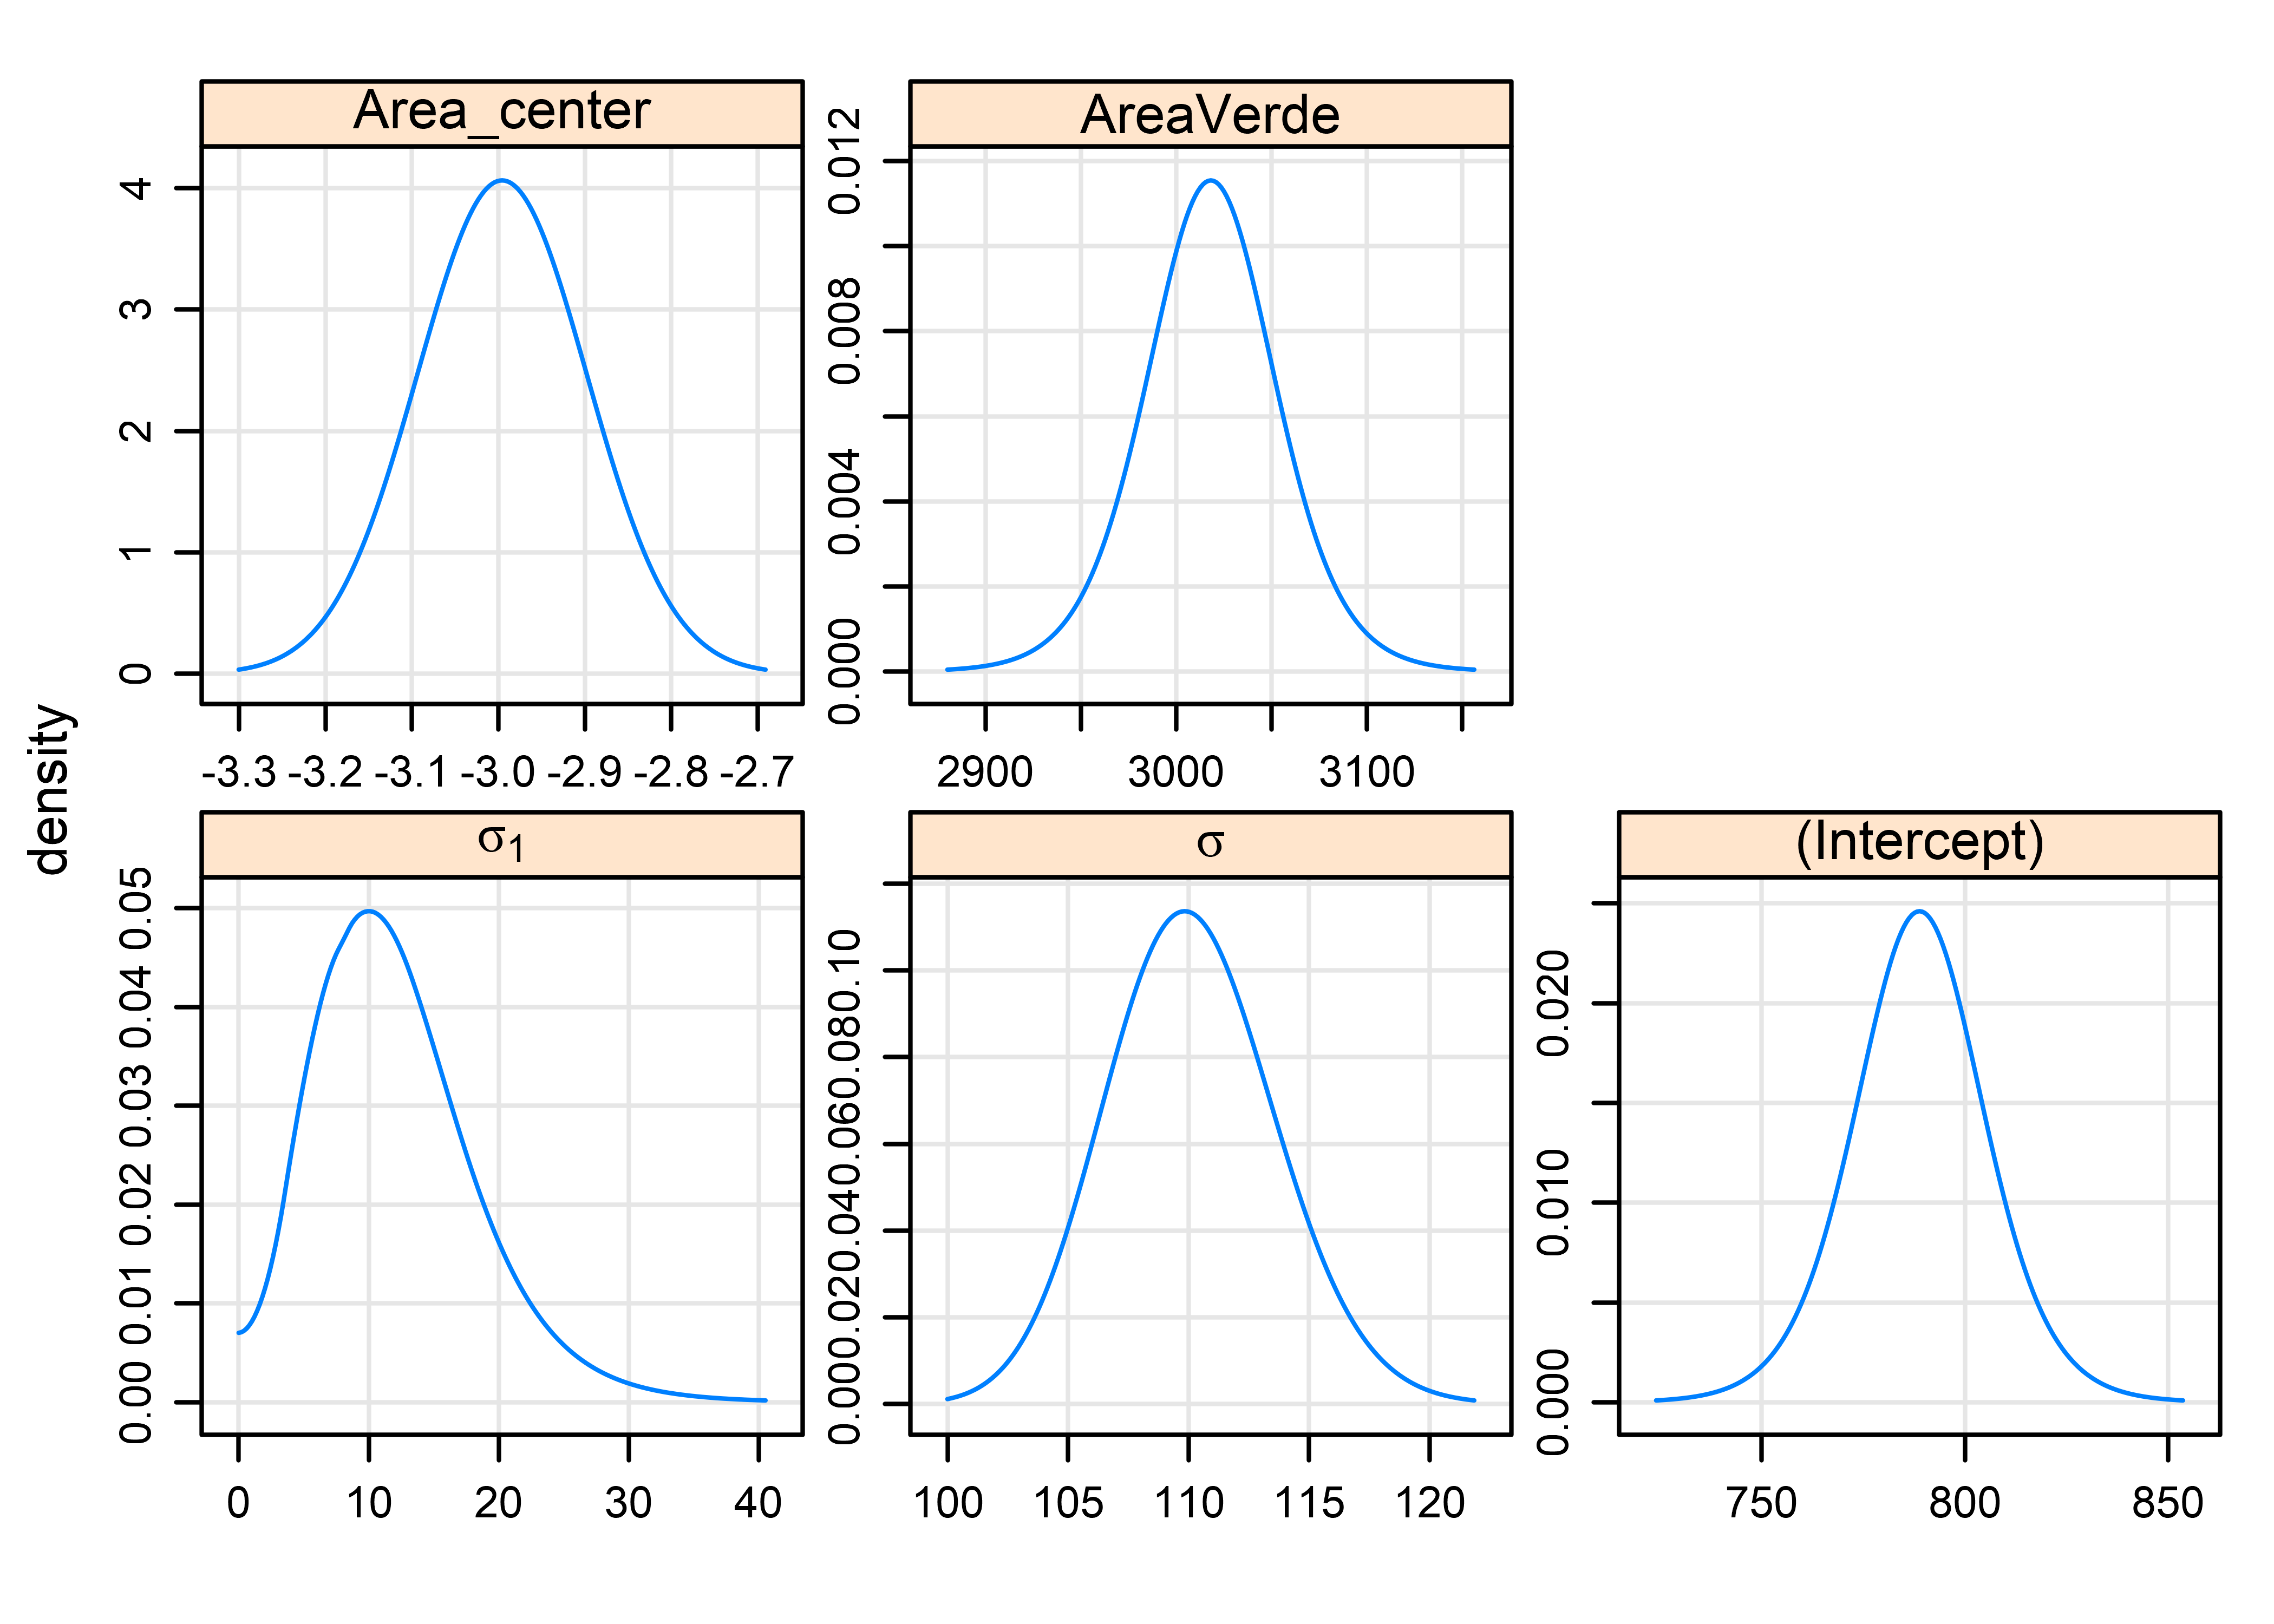
\includegraphics[width=0.66\linewidth]{images/pr1-1} 

}

\caption{Densidades dos parâmetros do modelo de efeitos mistos simples}\label{fig:pr1}
\end{figure}

\begin{figure}[H]

{\centering 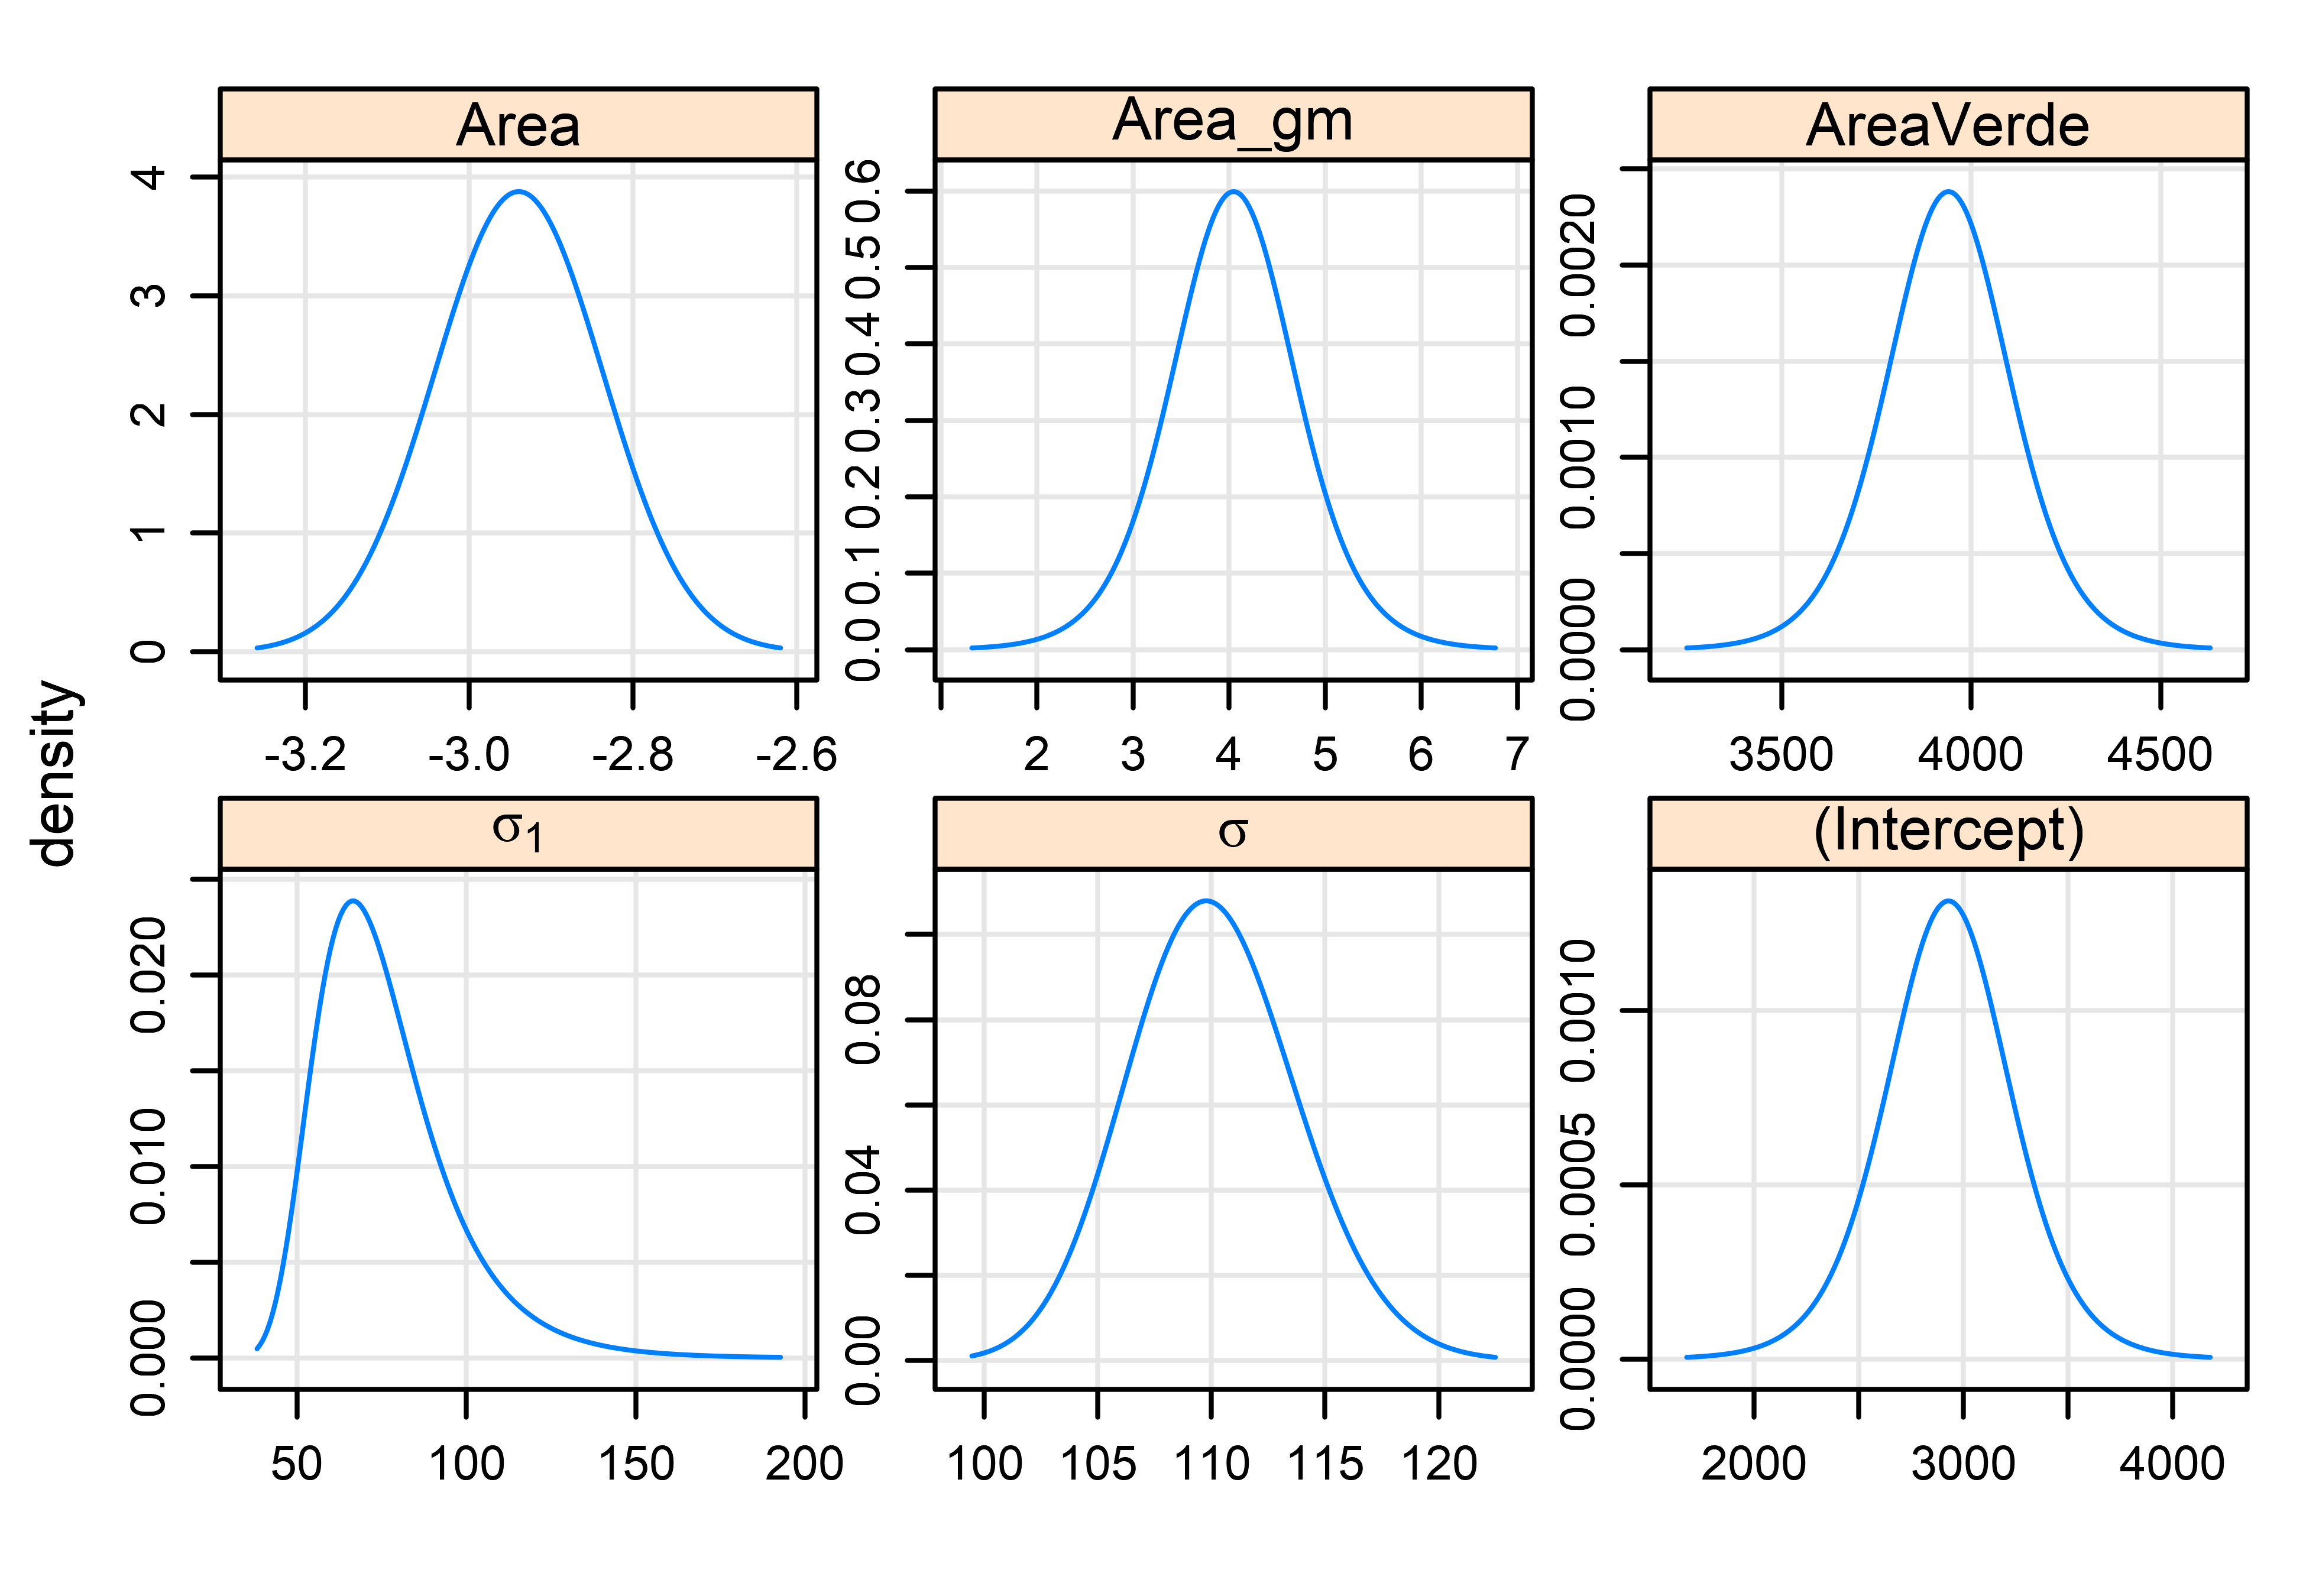
\includegraphics[width=1\linewidth]{images/pr2-1} 

}

\caption{Densidades dos parâmetros do modelo de efeitos mistos com variável de segundo nível}\label{fig:pr2}
\end{figure}

\hypertarget{previsuxe3o-de-valores}{%
\subsection{Previsão de Valores}\label{previsuxe3o-de-valores}}

Para ilustrar como os modelos mistos podem ser utilizados no contexto de
predição, foram elaboradas previsões no bairro H, que havia sido
propositalmente excluído no ajuste dos modelos mistos, com os diversos
modelos apresentados.

Também foram utilizados o modelo de efeitos fixos e o modelo misto com a
variável de segundo nível \(A_V\) para a previsão de valores de
lote-padrão para os diversos bairros, inclusive para o bairro H, não
utilizado para a confecção dos modelos mistos.

\hypertarget{previsuxe3o-de-dados-no-bairro-h}{%
\subsubsection{Previsão de dados no bairro
H}\label{previsuxe3o-de-dados-no-bairro-h}}

Na Figura \ref{fig:powerPlots} podem ser vistos os gráficos de poder de
predição para o modelo de efeitos fixos (A), para o modelo misto simples
(B), para o modelo misto com a variável de segundo nível (C) e para o
modelo misto com formulação de Mundlak (D). Como pode ser visto, todos
os modelos possuem poderes de predição praticamente equivalentes, com
exceção do modelo misto simples, onde a previsão de valores não pode ser
feita com precisão já que, como no modelo de efeitos fixos, este modelo
não tem parâmetros para prever valores em bairros não contemplados na
amostra. Para efetuar as previsões no bairro H, então, o modelo
considerou para a variável aleatória \(\upsilon\) o valor zero, ou seja,
o valor esperado da variável, o que levou a previsões incorretas em
relação aos valores simulados para aquele bairro.

\begin{figure}[H]

{\centering 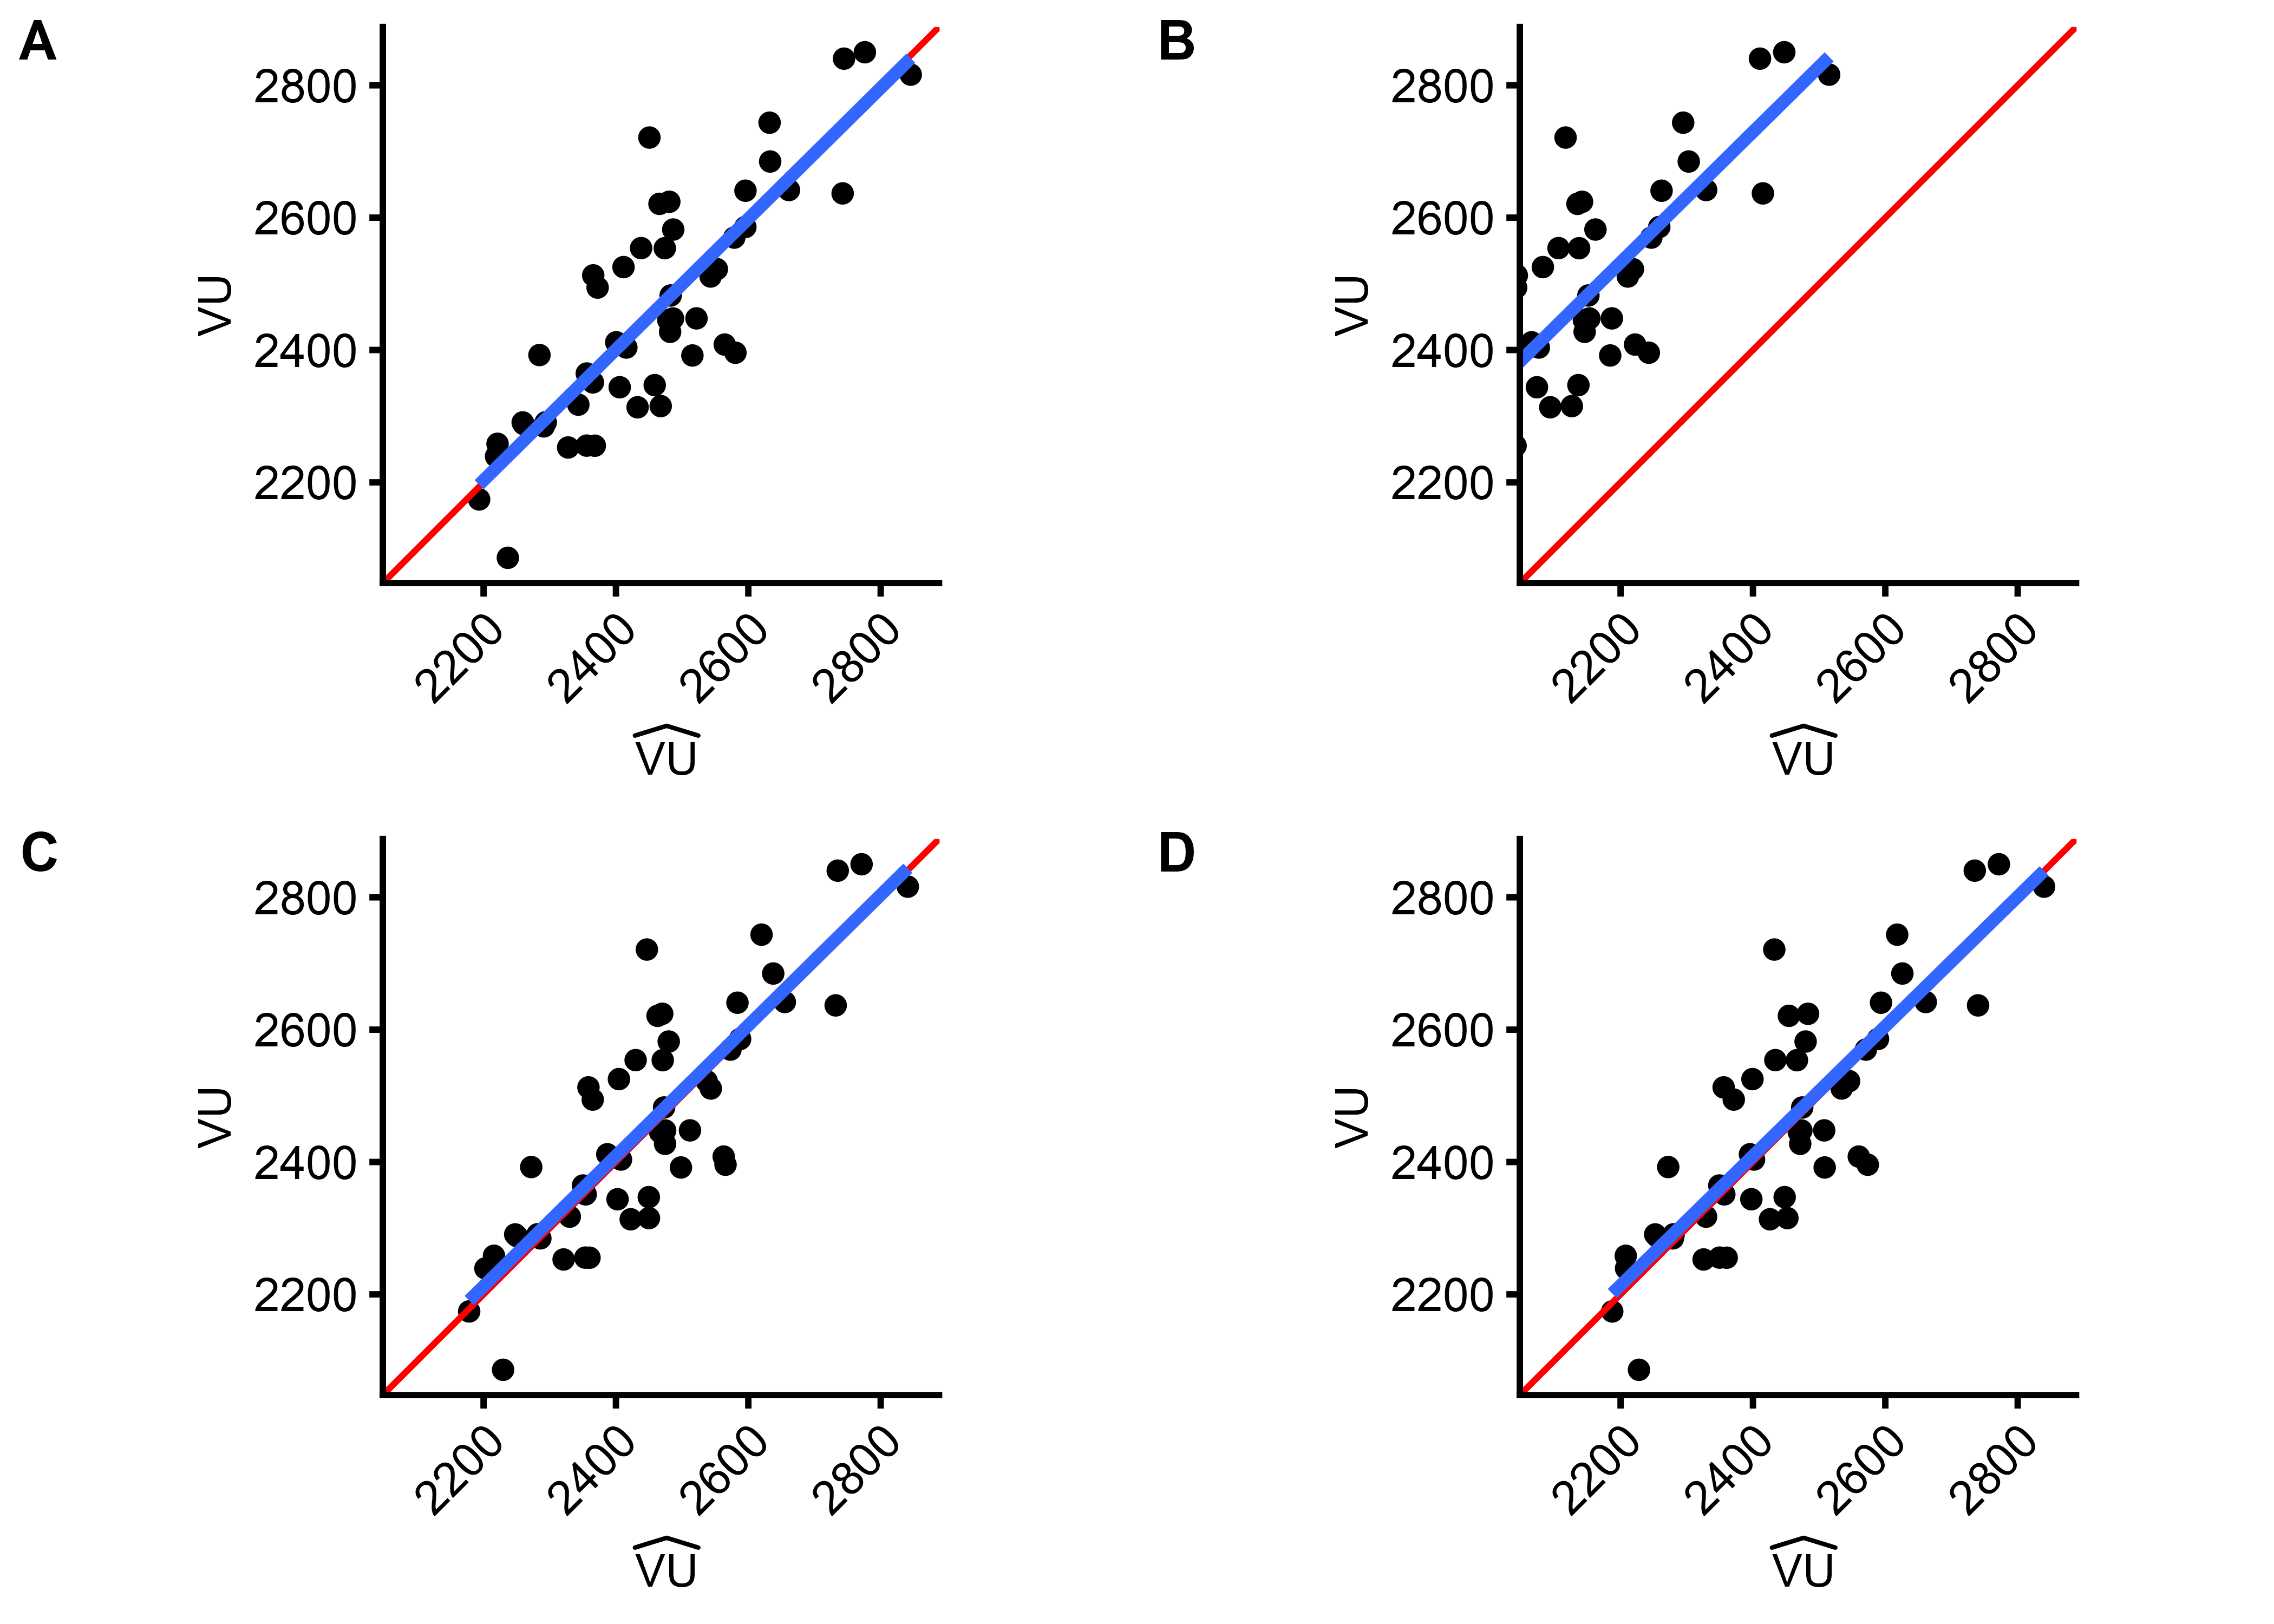
\includegraphics[width=1\linewidth]{images/powerPlots-1} 

}

\caption{Gráficos de poder de predição para cada modelo.}\label{fig:powerPlots}
\end{figure}

\hypertarget{previsuxe3o-de-valores-para-lotes-padruxe3o}{%
\subsubsection{Previsão de valores para
lotes-padrão}\label{previsuxe3o-de-valores-para-lotes-padruxe3o}}

Assim como a previsão de valores para os dados simulados para o bairro
H, conforme se mostrou no item anterior, é possível prever valores para
um lote-padrão nos diferentes bairros.

A tabela abaixo mostra os valores previsto pelos modelos para um
lote-padrão de 400 \(m^2\) nos diversos bairros:

\begin{longtable}[]{@{}ccc@{}}
\caption{Previsões para valores de Lote-Padrão nos diferentes
bairros.}\tabularnewline
\toprule
\begin{minipage}[b]{0.06\columnwidth}\centering
Bairro\strut
\end{minipage} & \begin{minipage}[b]{0.36\columnwidth}\centering
Modelo de efeitos fixos\strut
\end{minipage} & \begin{minipage}[b]{0.50\columnwidth}\centering
Modelo de efeitos mistos com variável de segundo nível\strut
\end{minipage}\tabularnewline
\midrule
\endfirsthead
\toprule
\begin{minipage}[b]{0.06\columnwidth}\centering
Bairro\strut
\end{minipage} & \begin{minipage}[b]{0.36\columnwidth}\centering
Modelo de efeitos fixos\strut
\end{minipage} & \begin{minipage}[b]{0.50\columnwidth}\centering
Modelo de efeitos mistos com variável de segundo nível\strut
\end{minipage}\tabularnewline
\midrule
\endhead
\begin{minipage}[t]{0.06\columnwidth}\centering
A\strut
\end{minipage} & \begin{minipage}[t]{0.36\columnwidth}\centering
1.379,72\strut
\end{minipage} & \begin{minipage}[t]{0.50\columnwidth}\centering
1.387,58\strut
\end{minipage}\tabularnewline
\begin{minipage}[t]{0.06\columnwidth}\centering
B\strut
\end{minipage} & \begin{minipage}[t]{0.36\columnwidth}\centering
1.530,98\strut
\end{minipage} & \begin{minipage}[t]{0.50\columnwidth}\centering
1.538,62\strut
\end{minipage}\tabularnewline
\begin{minipage}[t]{0.06\columnwidth}\centering
C\strut
\end{minipage} & \begin{minipage}[t]{0.36\columnwidth}\centering
1.696,18\strut
\end{minipage} & \begin{minipage}[t]{0.50\columnwidth}\centering
1.695,01\strut
\end{minipage}\tabularnewline
\begin{minipage}[t]{0.06\columnwidth}\centering
D\strut
\end{minipage} & \begin{minipage}[t]{0.36\columnwidth}\centering
1.891,57\strut
\end{minipage} & \begin{minipage}[t]{0.50\columnwidth}\centering
1.863,04\strut
\end{minipage}\tabularnewline
\begin{minipage}[t]{0.06\columnwidth}\centering
E\strut
\end{minipage} & \begin{minipage}[t]{0.36\columnwidth}\centering
1.982,52\strut
\end{minipage} & \begin{minipage}[t]{0.50\columnwidth}\centering
1.990,88\strut
\end{minipage}\tabularnewline
\begin{minipage}[t]{0.06\columnwidth}\centering
F\strut
\end{minipage} & \begin{minipage}[t]{0.36\columnwidth}\centering
2.133,79\strut
\end{minipage} & \begin{minipage}[t]{0.50\columnwidth}\centering
2.141,94\strut
\end{minipage}\tabularnewline
\begin{minipage}[t]{0.06\columnwidth}\centering
G\strut
\end{minipage} & \begin{minipage}[t]{0.36\columnwidth}\centering
2.313,13\strut
\end{minipage} & \begin{minipage}[t]{0.50\columnwidth}\centering
2.303,78\strut
\end{minipage}\tabularnewline
\begin{minipage}[t]{0.06\columnwidth}\centering
H\strut
\end{minipage} & \begin{minipage}[t]{0.36\columnwidth}\centering
2.457,33\strut
\end{minipage} & \begin{minipage}[t]{0.50\columnwidth}\centering
2.450,14\strut
\end{minipage}\tabularnewline
\begin{minipage}[t]{0.06\columnwidth}\centering
I\strut
\end{minipage} & \begin{minipage}[t]{0.36\columnwidth}\centering
2.597,51\strut
\end{minipage} & \begin{minipage}[t]{0.50\columnwidth}\centering
2.598,88\strut
\end{minipage}\tabularnewline
\begin{minipage}[t]{0.06\columnwidth}\centering
J\strut
\end{minipage} & \begin{minipage}[t]{0.36\columnwidth}\centering
2.741,39\strut
\end{minipage} & \begin{minipage}[t]{0.50\columnwidth}\centering
2.747,09\strut
\end{minipage}\tabularnewline
\begin{minipage}[t]{0.06\columnwidth}\centering
K\strut
\end{minipage} & \begin{minipage}[t]{0.36\columnwidth}\centering
2.901,56\strut
\end{minipage} & \begin{minipage}[t]{0.50\columnwidth}\centering
2.901,56\strut
\end{minipage}\tabularnewline
\bottomrule
\end{longtable}

\hypertarget{intervalos-de-prediuxe7uxe3o}{%
\subsubsection{Intervalos de
Predição}\label{intervalos-de-prediuxe7uxe3o}}

No caso dos modelos mistos, os intervalos de predição são calculados
separadamente para cada efeito. Na tabela \ref{tab:pred1} podem ser
vistos os intervalos de predição (@80\%) para o lote-padrão no bairro G.
A primeira linha mostra o intervalo total de predição combinado para os
dois efeitos. A segunda linha mostra o intervalo de predição para o
efeito aleatório (Bairro) e a terceira linha mostra o intervalo de
predição para o efeito fixo.

\begin{table}[H]

\caption{\label{tab:pred1}Intervalo de Predição com o modelo de efeitos mistos simples.}
\centering
\fontsize{10}{12}\selectfont
\begin{tabular}[t]{lrrrr}
\toprule
Efeito & Valor Central & Limite Superior & Limite Inferior & Observações\\
\midrule
\rowcolor{gray!6}  combined & 2.317,3 & 2.560,2 & 2.065,9 & 1\\
Bairro & 194,1 & 333,6 & 56,3 & 1\\
\rowcolor{gray!6}  fixed & 2.121,5 & 2.364,9 & 1.882,1 & 1\\
\bottomrule
\end{tabular}
\end{table}

A tabela \ref{tab:pred2} mostra o intervalo de predição para o
lote-padrão no bairro H.

\begin{table}[H]

\caption{\label{tab:pred2}Intervalo de Predição com o modelo de efeitos mistos com variável de segundo nível}
\centering
\fontsize{10}{12}\selectfont
\begin{tabular}[t]{lrrrr}
\toprule
Efeito & Valor Central & Limite Superior & Limite Inferior & Observações\\
\midrule
\rowcolor{gray!6}  combined & 2.449,7 & 2.600,0 & 2.300,7 & 1\\
Bairro & -1,7 & 149,4 & -136,8 & 1\\
\rowcolor{gray!6}  fixed & 2.447,1 & 2.587,7 & 2.301,4 & 1\\
\bottomrule
\end{tabular}
\end{table}

Para efeitos de comparação, a tabela \ref{tab:pred3} mostra o intervalo
de predição para o bairro H calculado com o modelo de efeitos fixos.

\begin{table}[H]

\caption{\label{tab:pred3}Intervalo de Predição com o modelo de efeitos fixos}
\centering
\fontsize{10}{12}\selectfont
\begin{tabular}[t]{lrrr}
\toprule
Efeito & Valor Central & Limite Superior & Limite Inferior\\
\midrule
\rowcolor{gray!6}  Fixo & 2.457,3 & 2.598,5 & 2.316,2\\
\bottomrule
\end{tabular}
\end{table}

Nota-se que os intervalos de predição do modelo de efeitos fixos
apresentados na tabela \ref{tab:pred3} e o intervalo de predição total
combinado (linha 1) do modelo de efeitos mistos com variável de segundo
nível praticamente se equivalem. Deve-se lembrar, porém, que para o
modelo de efeitos fixos foram utilizados 10\% mais dados e que o modelo
de efeitos mistos não utilizou qualquer dado amostral proveninente do
bairro H.

\hypertarget{conclusuxe3o-e-sugestuxe3o-para-trabalhos-futuros}{%
\section{Conclusão e sugestão para trabalhos
futuros}\label{conclusuxe3o-e-sugestuxe3o-para-trabalhos-futuros}}

A aplicação da modelagem mista ou hierárquica na Engenharia de
Avaliaçãoes pode ser feita das mais diversas maneiras, desde a aplicação
em avaliações de precisão, até a avaliação em massa para fins
tributários, assim como para confecção de índices de preços de imóveis.

Neste trabalho foi mostrado como a Engenharia de Avaliações pode se
valer da modelagem hierárquica ou mista para a confecção de PVG's, com a
utilização de modelos com interceptos aleatórios, especialmente para
estimação de valores para lotes-padrão em agrupamentos não presentes na
amostra, através da utilização de variáveis de segundo nível que
\emph{expliquem} a variabilidade entre os bairros ou outros
agrupamentos. Tais modelos são mais complexos e ao mesmo tempo
elegantes, dividindo a variabilidade em diversos níveis, deixando claro
ao analista de onde advém a variabilidade dos preços.

Embora a modelagem hierárquica seja considerada mais elegante do que a
modelagem de efeitos fixos, deve-se ter em conta que a elaboração de
modelos mistos sem variáveis de segundo nível, como é comum encontrar na
literatura, não é tão interessante e quase nada agrega a uma melhor
explicação do fenômeno estudado. Deve até haver uma melhora na estimação
com os modelos mistos caso os dados de alguns agrupamentos estejam em
número reduzido, mas o ideal é utilizar as formulações mais complexas da
modelagem hierárquica de maneira a explorar ao máximo este tipo de
modelagem.

Na análise de dados em seção transversal, como na elaboração de
avaliações de precisão ou na elaboração de PVG's, deve ser utilizada,
preferencialmente, a formulação de Mundlak, enquanto para dados em
painéis, como na confecção de índices de preços de imóveis, deve ser
preferencialmente utilizada a formulação REWB.

Na modelagem hierárquica ainda é possível incorporar outras hipóteses
úteis, além dos interceptos aleatórios, como também coeficientes
aleatórios, o que deve ser tema de outro trabalho.

Outra possibilidade é a modelagem em mais níveis hierárquicos. Não
apenas os imóveis podem ser agrupados em bairros, mas também os bairros
podem, por sua vez, ser agrupados em macrozonas urbanas, assim como
estas podem ser agrupadas em cidades, as cidades em regiões e assim por
diante. A execução de modelos tão complexos com efeitos fixos é
praticamente inviável.

Outra possibilidade é a modelagem dos dados ao longo do tempo, o que
possibilita a sua utilização para a confecção de índices de preços de
imóveis.

\hypertarget{referuxeancias}{%
\section*{Referências}\label{referuxeancias}}
\addcontentsline{toc}{section}{Referências}

\hypertarget{refs}{}
\leavevmode\hypertarget{ref-Batesbook}{}%
BATES, D. \textbf{Lme4: Mixed-effects modeling with R}. 2010.

\leavevmode\hypertarget{ref-Bates}{}%
BATES, D.; MÄCHLER, M.; BOLKER, B.; WALKER, S. Fitting linear
mixed-effects models using lme4. \textbf{Journal of Statistical
Software}, v. 67, n. 1, p. 1--48, 2015.

\leavevmode\hypertarget{ref-bell2019}{}%
BELL, A.; FAIRBROTHER, M.; JONES, K. Fixed and random effects models:
Making an informed choice. \textbf{Quality and Quantity}, v. 53, p.
1051--1074, 2019.

\leavevmode\hypertarget{ref-bell2015}{}%
BELL, A.; JONES, K. Explaining fixed effects: Random effects modeling of
time-series cross-sectional and panel data. \textbf{Political Science
Research and Methods}, v. 3, n. 1, p. 133--153, 2015. Cambridge
University Press.

\leavevmode\hypertarget{ref-polonia}{}%
CICHULSKA, A.; CELLMER, R. Analysis of prices in the housing market
using mixed models. \textbf{Real Estate Management and Valuation}, v.
26, n. 4, p. 102--111, 2018.

\leavevmode\hypertarget{ref-clark2019shrinkage}{}%
CLARK, M. Shrinkage in mixed effects models. \textbf{Michael Clark},
2019. Disponível em:
\textless{}\url{https://m-clark.github.io/posts/2019-05-14-shrinkage-in-mixed-models/}\textgreater..

\leavevmode\hypertarget{ref-droubi2019}{}%
DROUBI, L. F. P.; ZILLI, C. A.; HOCHHEIM, N. Centralização e
escalonamento de dados amostrais: Prós, contras e aplicação na
engenharia de avaliações. In: XX Congresso Brasileiro de Avaliações e
Perícias. \textbf{Anais\ldots{}}, 2019. Florianópolis: COBREAP.

\leavevmode\hypertarget{ref-R}{}%
R CORE TEAM. \textbf{R: A language and environment for statistical
computing}. Vienna, Austria: R Foundation for Statistical Computing,
2020.

\end{document}
